\documentclass[twoside]{bhamthesis}

\usepackage{graphicx}
\usepackage{amssymb}
\usepackage{appendix}
\usepackage{biblatex}
\usepackage{listings}

\bibliography{pcp620_report_2017.bib}

\title{Solar System Explorer - An Incremental Game}
\author{Philip Prior (0920420)}
\supervisor{Hayo Thielecke}
\degree{MSc Computer Science}
\department{Computer Science}

\renewcommand\thesection{\arabic{section}}
\DefineBibliographyStrings{english}{%
  bibliography = {References},
}
\raggedbottom

\lstset{
	basicstyle=\ttfamily\footnotesize,
          breaklines=true
          }

\begin{document}
\maketitle
\clearemptydoublepage

\tableofcontents

\listoffigures
\addcontentsline{toc}{section}{\listfigurename}

\begin{abstract}

This report details the design and implementation of a software engineering project to create a space exploration themed incremental game. The challenge was to introduce a degree of realism to the representation of space beyond that in similar products from the incremental games market.

The game was created using languages that made it suitable for delivery via a Web browser, using an incremental software development lifecycle and focusing on prototyping for testing during development.

A game named “Solar System Explorer” was produced, successfully incorporating several planned features including those required to meet the definition of an incremental game.

Suggestions are also provided herein as to the further development of the product beyond the timescale of this particular project.

\end{abstract}

\begin{acknowledgments}
I would like to thank my supervisor Hayo Thielecke for his advice and support in the completion of this project.

Thanks also to Uday Reddy and the rest of the teaching staff at the University of Birmingham's School of Computer science for their support and guidance.

I would like to acknowledge the contributions of the NASA and ESO teams through the use of their imagery to produce textures for both the planets and milky way.

Finally I would like to extend my appreciation to the individuals, classmates and acquaintances who assisted me in testing and providing feedback on my product.
\end{acknowledgments}

\section{Introduction}
\markboth{Introduction}{Introduction}

The aim of the work described in this report was to create a web based incremental game that seeks to provide a more realistic representation of the solar system than in present in other products in the genre.

It is an oft discussed issue that scientific theories and data suffer from a distortion of representation and a skew in perception in both popular media and the arts. This is common across all forms of media, from classic painting to modern forms of entertainment such as video games. Such misrepresentation hinders the public understanding of natural phenomena and is arguably more effective at (mis)educating than traditional classroom based learning. In discussing education related to the theory of evolution Brian Alters notes that, "Not only does the general public lack an understanding of evolution but so does a considerable proportion of college graduates." \cite{alters_perspective:_2002}. He goes on to explain that formal education has a very tough time combatting the informal, and often incorrect, learning.

\begin{figure}[h!]
  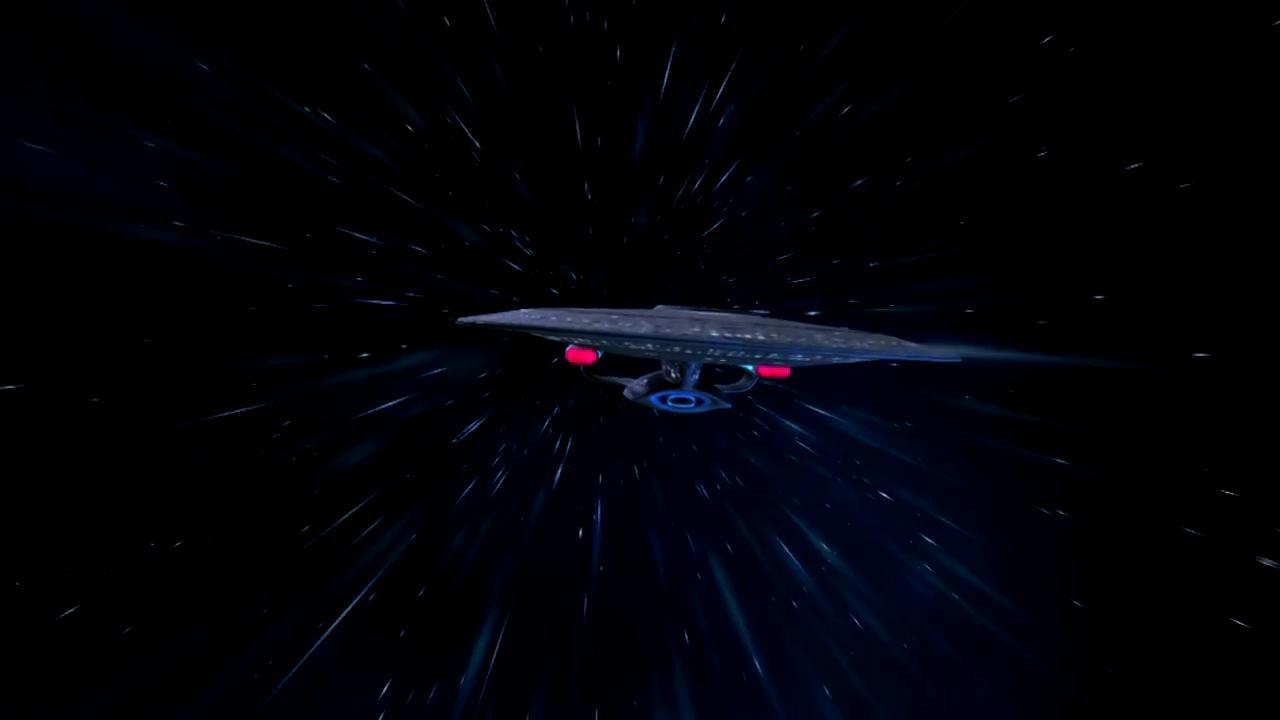
\includegraphics[width=\linewidth]{images/star_trek_warp.jpg}
  \caption{A typical media image of interstellar travel, Star Trek's Enterprise travelling at 'Warp Speed' {\cite{_gamescom_2011}}}
  \label{fig:star_trek}
\end{figure}


This is very evident in the discipline of astrophysics, where decades of science-fiction and science-fantasy artistic representation and storytelling have resulted in a very poor public understanding of the physical solar system, the technologies available for space exploration and the possibilities of interplanetary travel. So much so that lexicons of terms, and scales for the description of, the relative 'hardness' of such representations have sprung up in the scientific, engineering and media production communities \cite{_mohs_????}. Whilst fiction writers describe the use of impossible faster-than-light 'warp drive' technologies to navigate across interstellar distances, actual scientists are still working on the hugely challenging problem of reaching the nearest neighbouring planets in our own solar system.

This is not to belittle the influence and inspiration to be had from speculative fiction, the number of technologies predicted or inspired by writers like Isaac Asimov or Arthur C. Clarke are well documented. However there is a great opportunity in the media representation of astrophysical phenomena to provide for a valuable learning experience at the same time as being entertained. To this end it was considered a worthy pursuit to create a compelling video game in a genre known as 'incremental gaming', also known as 'idle gaming' or 'clicker gaming'. This genre takes advantage of such psychological factors  as accumulation desire and loss aversion placing the player in an environment that constitutes a simple Skinner box \cite{carlson_psychology:_2009}.

Most games of this type are delivered either as a mobile phone app or as a browser based 'web game', possibly the most famous of which is Cow Clicker, a product that parodied the repetitive gameplay of the Farmville games from publisher Zynga.

\begin{figure}[h!]
  
\includegraphics[width=\linewidth]{images/cowclicker.jpg}
  \caption{Infamous parody 'clicker' game Cow Clicker {\cite{_games_2016}}}
  \label{fig:cowclicker}
\end{figure}

Such a product is simple enough for the core mechanics to have been achievable within the timeframe of this project whilst also providing an opportunity to address the issue of realistic representation. It is not expected that any product would be able to give a completely realistic model of a detailed astrophysics problem, but some degree of relative realism could be attained that goes beyond the usual fare in this genre of entertainment media.

\newpage
\noindent
This report will detail the creation of the Solar System Explorer incremental game.

\medskip
The analysis and specification section discusses the initial phases of development, detailing the overall goals for the software product and giving some examples of the requirements that formed the basis for the direction of the product's development.

\medskip
In the design section we find a more in depth explanation as to the choices involved in the gameplay and game logic design, an explanation as to the rationale behind the orbital models used and the programming languages selected for development. Finally a brief discussion as to structure of the product and how this relates to the host architecture.

\medskip
The implementation section gives some detail about the data types and structures used in the project with justifications for why these were chosen, an example method demonstrating a mathematical transformation in 3 dimensional space and a brief description of how the objects in the 3D environment were deployed. This section also incorporates a description of the testing methods employed throughout the development process.

\medskip
There is a discussion of conventions in the user interface section, how these relate to the choices made in designing the Solar System Explorer's look and feel and also detailing some of the interface's behaviour.

\medskip
The project management section lists the tools and methodology used alongside a brief review of how successfully these were utilised.

\medskip
The results and evaluation section contains a breakdown of some qualities of the final delivery along with reflections on user responses to the product.

\medskip
This is followed by a discussion of the strengths and weaknesses of the product, how these relate to the relative success of the project and what further improvements may have been made given further time.

\medskip
Finally a conclusion is offered as to how the product addresses the problems described in this introduction.

\section{Analysis and specification}
\markboth{Analysis and specification}{Analysis and specification}

The problem was initially analysed by investigating other products in the genre, specifically focusing on a web browser game entitled 'Spaceplan' by Jake Hollands. The features and mechanical gameplay elements of these were broken down into simple lists and categorised to find conventions that span the genre. This primarily involved a card-sort exercise, derived from the technique utilised in usability design.

Given the mechanics of the incremental games model some of these features were inherent, yet some were not, for example the necessity of including some form of text based feedback at key points in progress. This text could take the form of a narrative as in a product akin to Spaceplan \cite{hollands_spaceplan_2017} or as a goal/achievement flag as seen in Cookie Clicker \cite{ortiel_cookie_2017}.

\begin{figure}[h!]
  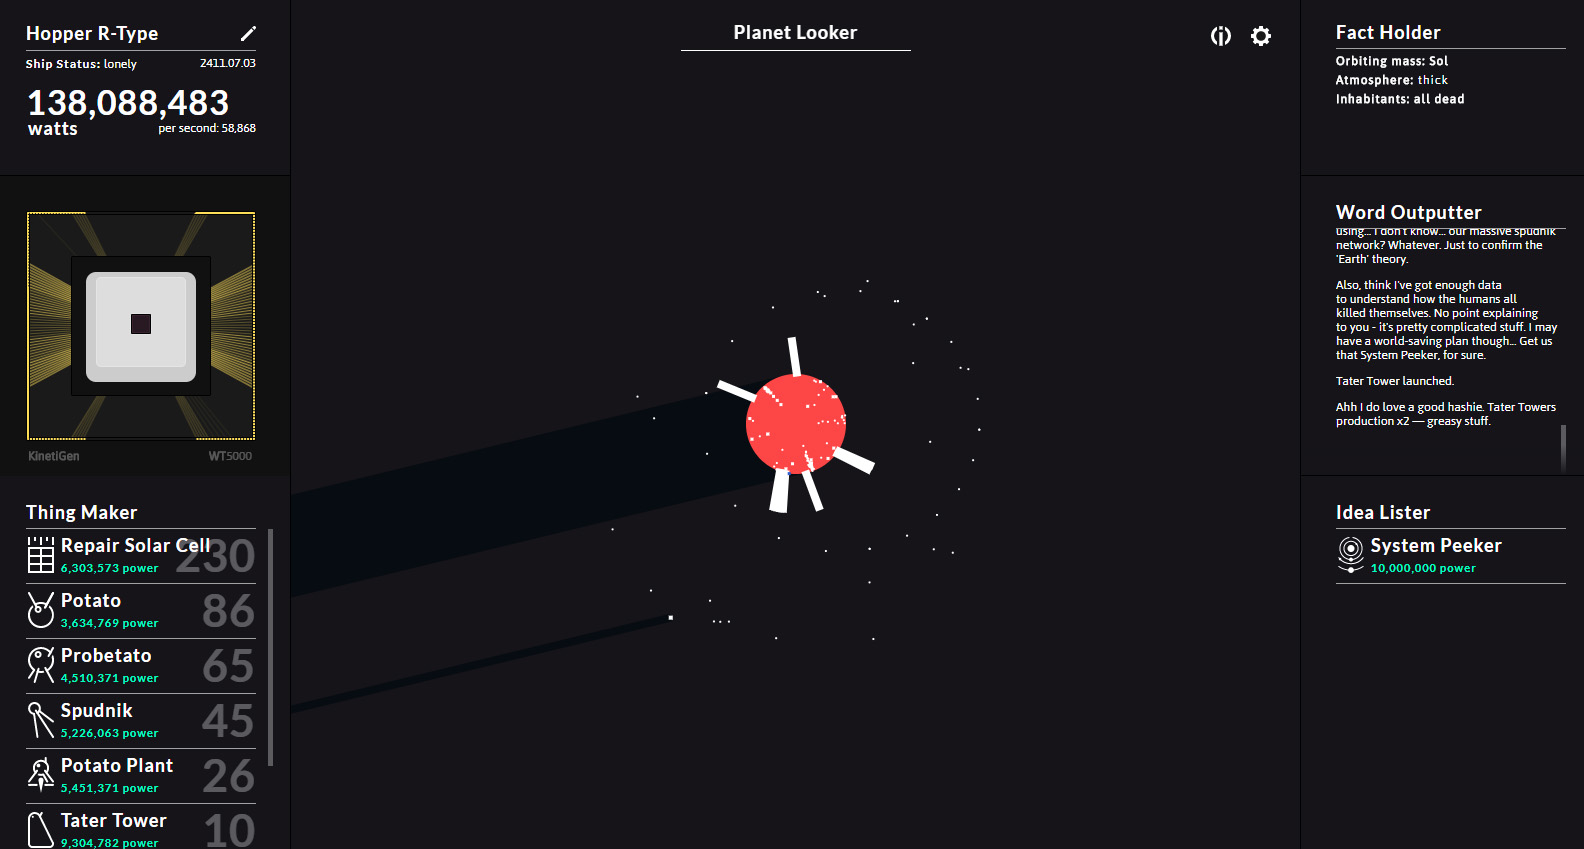
\includegraphics[width=\linewidth]{images/spaceplan.jpg}
  \caption{Example incremental game: Spaceplan}
  \label{fig:spaceplan}
\end{figure}

As the project did not follow a standard software-development lifecycle as detailed in the project management section of this report, but instead followed a process that relates most closely to a hybrid of Agile methodologies (rapid iteration, not documentation-centric, yet eschewing test-driven-development) and the media production workflow common to games production (concept, pre-production, production, post and distribution phases), a simple non-exhaustive of requirements was created, including some non-functional requirements based on the heuristics provided in the GameFlow model \cite{sweetser_gameflow_2012}, adapted from their approach to real-time-strategy gaming.

Very few statistics were available on the demographics of incremental game players as this information is not typically recorded as a part of play and they are usually relegated to a broader category including other 'casual games' when investigated in games research papers. With this apparent paucity of available data, very little could be done to target or analyse the requirements of any specific user group.

\subsection{General specification}


Solar System Explorer is a web browser based game of the incremental game genre. Its mechanics are based on the acquisition of resources represented by one or more numbers that increment continuously, even whilst the player of the game is idle.

There are mechanisms in the game to increase the rate at which these numbers increment by expending some of the previously gained resource. The game is themed around the exploration of our solar system, modelled on real measurements provided by astrophysics organisations. It uses scientific terminology and representations of data that are reasonably accurate to the real world and any mechanic or terminology that has a basis in only hypothesis or speculative fiction is clearly explained as such.

The game provides a semi-realistic visual representation of the planets and their orbits, specifically focusing on representations of scale and distance, with as little abstraction as possible.

The interface for the game is a 2-dimensional overlay on a 3-dimensional visualisation and the only tool for interaction required is of the pointer type (mouse, trackpad, touchscreen, etc). Player interaction results in visual feedback relating to the rate of resource gain, contextual information about optional increases to the rate of resource gain and visual feedback via the 3-dimensional graphical representation.

The game starts with only the Earth visible and the overall goal of the game is to unlock access to view all of the planets in the solar system along with related scientific data. When all planets are unlocked, the player is rewarded with a special access code for a sequel game based on interstellar travel.

\subsubsection{Fallback specification}
Should there have been inadequate time for delivery of the full specification above, the expected delivery should have been, at a minimum, a text based implementation of the game mechanics with a graphical representation of the solar system to serves as an aesthetic accompaniment.

\subsection{Example requirements}
Presented here is a short selection of functional and non-functional requirements, typical to this kind of software engineering project, that were elicited during the early phases of development of Solar System Explorer.

\subsubsection{Functional requirements}

Logic requirements
\begin{itemize}
\item[] LOFR001 - The game must automatically increment, by a set amount, each available resource on a periodic basis set by the framerate.
\item[] LOFR002 - The game must automatically update, on a periodic basis set by the framerate, the x,y,z coordinate position of stellar bodies
\item[] LOFR003 - A button for each type of resource, when clicked, must add a fixed amount of said resource to the general pool available to the player
\end{itemize}

\noindent
UI requirements
\begin{itemize}
\item[] UIFR001 - The minimum necessary resolution for interacting with the game UI must not exceed a resolution of 1280 x 720 pixels
\item[] UIFR002 - Elements of the interface that are not interactive should not be selectable within the browser window
\item[] UIFR003 - Interactive elements of the game UI (clickable) must trigger a change in state of the mouse cursor on a hover condition
\end{itemize}

\subsubsection{Non-functional requirements}

\noindent
Performance requirements
\begin{itemize}
\item[] PFNFR001 - The total time taken to download the client code and assets over a domestic 8mbps+ broadband connection should not exceed 5 seconds
\item[] PFNFR002 - All interactive user interface options, when triggered, should provide some form of visual feedback for the user in under 200ms
\item[] PFNFR003 - Any animation in the user interface should maintain a display framerate of greater than 15 frames per second on a mid-range client machine
\end{itemize}

\noindent
Compliance requirements
\begin{itemize}
\item[] CONFR001 - All markup code should comply with W3C standards as per the HTML 5 recommendation
\item[] CONFR004 - All imagery should be right cleared for use in an educational/non-profit product
\item[] CONFR005 - Any licenced content should be appropriately acknowledged as per the licensing requirements
\end{itemize}

\subsection{Example game specific requirements}
In addition to the typical requirements expected in a software engineering project, game design demands the inclusion of gameplay specific non-functional requirements. These are often hard to define with complete specificity so are less easily measured. Typically in modern development they will be evaluated at the point of beta testing the product or as an ongoing concern post-release, evaluated through user feedback and altered by deploying patches (sometimes descibed as being 'in permanent beta'). The GameFlow model \cite{sweetser_gameflow_2017}, whilst not specifically created for the genre of incremental gaming, provided some suitable guidance and was used as an example for designing gameplay requirements.


\bigskip
\noindent
Gameplay requirements
\begin{itemize}
\item[] GPNFR001 - The game should conform to genre conventions to allow the player to have an inherent understanding of the game
\item[] GPNFR002 - The gameplay should be easy to pick up for new players
\item[] GPNFR003 - The game should gradually introduce new upgrades and items so that the player learns a little at a time
\item[] GPNFR004 - The game should consistently reward the player for their effort, and motivate them to keep playing, through story developments
\end{itemize}



\section{Design}
\markboth{Design}{Design}

\subsection{Game design}

In an article entitled 'Numbers Getting Bigger: What Are Incremental Games, and Why Are They Fun?' \cite{king_numbers_2015} it is identified that the fundamental aspects of design that define an incremental game are:
\begin{itemize}
\item the presence of at least one currency or number, 
\item which increases at a set rate, with no or minimal effort, 
\item and which can be expended to increase the rate or speed at which it increases. \ldots
\end{itemize}
 
Surveying the various online catalogues of 'incremental', 'clicker' and 'idle' games provides a rich tapestry of examples of this genre of game, each of which follows these general rules. These indeed consitute the necesary terms for defining a genre as a taxonimic ideal based on identifiable characteristics \cite{clarke_why_2017}.

Given that the aim of this project was to create an incremental game, but with a more realistic representation of the realities of space exploration, it seemed that the challenge was to marry a very simple gaming mechanic with a very complex field of science. Compromises would have to be made, as this was not going to be a full space physics simulator in the style of a full commercial entertainment package like 2015's Kerbal Space Program \cite{squad_kerbal_2015}, yet some degree of realism would have to be maintained.

\begin{figure}[h!]
  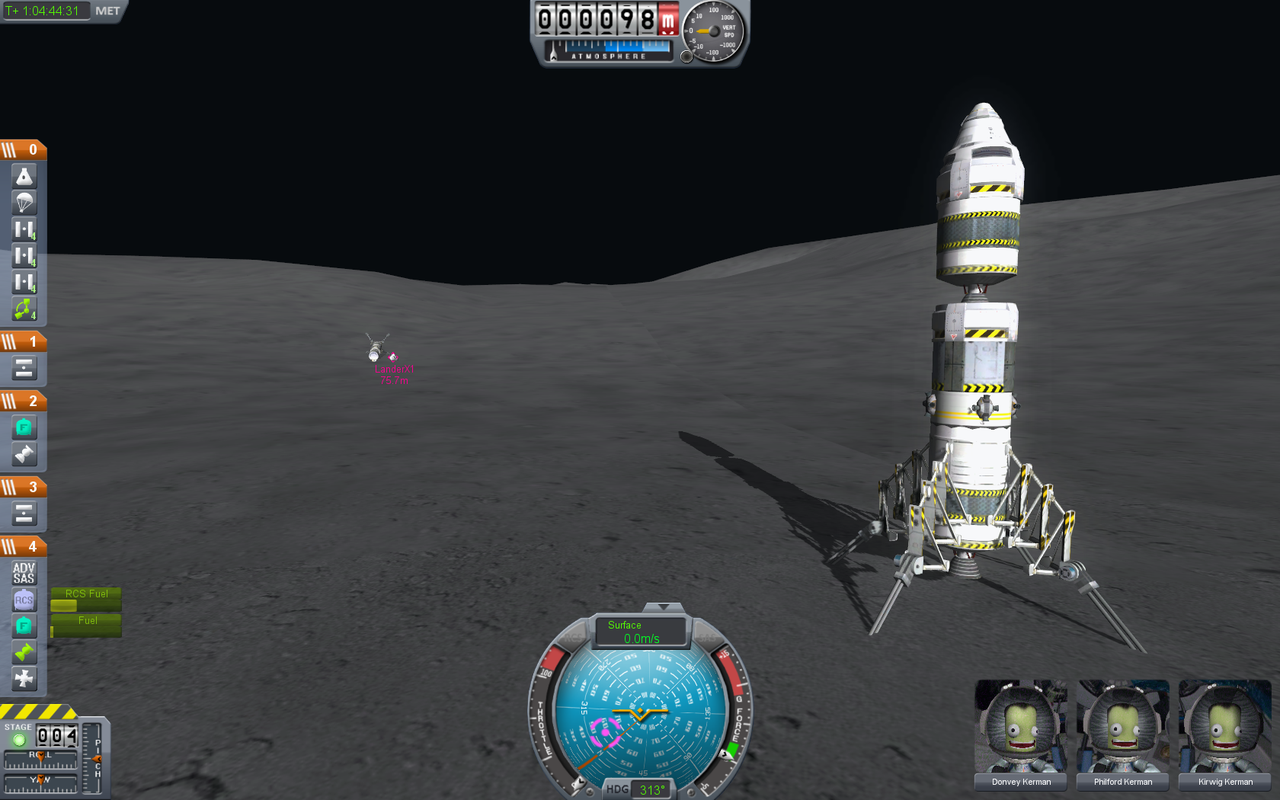
\includegraphics[width=\linewidth]{images/ksp.png}
  \caption{Space physics sandbox game: Kerbal Space Programme {\cite{tang_kerbal_2014}}}
  \label{fig:ksp}
\end{figure} 

Initial designs focused on the interaction of 4 different competing resources, with consideration for aspects that otherwise are under represented in science fiction gaming, such as political will and popular support. However, even paper prototypes of these ideas became riddled with issues e.g.complexity stretching beyond that found elsewhere in the genre, approaching that of '4X' games \cite{gunn_taxonomy_2009} and user interface design issues due to a lack of screen real estate when following the single screen convention of the genre. It was eventually decided to settle on a dual resource system representing different forms of energy income with some necessary level of abstraction. The concept of nuclear and photonic sources of energy would form the basis for this resource system, representing a duality not only of a scientific nature, but of an ethical one also. Players could choose to focus on 'dirty' nuclear energy for fast progress at the start of the game or 'clean' photonic energy for faster progress towards the end.

The functionality that would allow for the 'increase in rate or speed' would provide an opportunity to add context and detail by allowing access to a system of tiered upgrades (commonly referred to in gaming parlance as a 'tech tree') which would use actual scientific and technological terms.

By navigating up the tree of upgrades the player would gradually explore different planets in the solar system, revealing an attractive graphical display of each accompanied by on-screen information about the planet, its orbital data and some other facts relating to the realities of exploring said planet. One example of this would be to limit the upgrades available on Jupiter to orbital items only, given the gaseous nature of and the high gravity conditions that exist close to the surface.

The overall aim of the game in its full form would be to reveal all planets in the solar system and unlock an access code for a sequel game based on the concept surrounding interstellar, rather than interplanetary, exploration and travel. The game would not terminate at this point however, leaving the user to explore the interface, continue to accrue resources and look over the information presented during the course of the experience.

Consideration was given to producing a 2-dimensional graphical represention of the planets as this was a common feature of other games in the genre, however it seemed possible to present a greater degree of realism by modelling the solar system in a 3-dimensional space. A 2-dimensional overlay or 'Heads Up Display' (HUD) would allow for interaction and the presentation of data to the player. To further enhance the sense of realism, where possible, image assets would be obtained from photographic libraries rather than relying on artistic visualisations.


\subsection{Orbital models}
Initial investigations into methods for creating models to represent the solar system led to quite a few simulations of gravitational attraction. These ranged from simple bouncing balls to mutiple moving objects accelerating according to the laws of gravitation.

Several of these were (re)created as exploratory prototypes in the Processing sketchbook IDE, however it rapidly became apparent that these models had certain limitations and that to ensure continuous motion any bodies were subject to positional limits. It also became clear that to calculate the attraction of multiple bodies would not be as simple. This is referred to in physics as the 'three body problem' and is probably best understood by the analogy of calculating the movements of the Sun, Earth and Moon with each affecting the other. Texts dating back to 1887  by the mathematician Heinrich Bruns demonstrated that there were no general solutions to the three body problem, only special cases such as Lagrange points \cite{oconnor_bruns_????}. This explains the need to reduce gravitional models to two bodies or to artificially impose limits on the motion of the objects in any such model.

\begin{figure}[h!]
  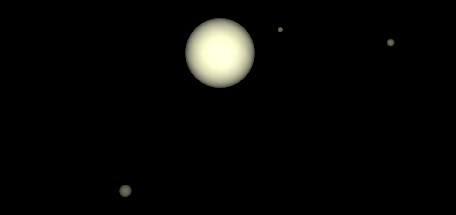
\includegraphics[width=\linewidth]{images/grav_proto.png}
  \caption{Early 3D prototype of two body gravitational attraction, created in Processing.}
  \label{fig:grav_proto}
\end{figure} 

Further reading around the topic of modelling orbits \cite{dvorak_chaos_2005}  led back to Kepler's laws of motion, which fit a simulation of this type far better. By modelling orbits as ellipses, bearing in mind that planetary orbits in our solar system are close to circular, a more consistent visualisation of orbital motion could be produced using simpler trigonometric calculations. This would ensure that unlike the gravitational motion based on attraction and acceleration, there was no risk of errors over a longer period of time where a body may come to rest or similar erroneous representation.



\subsection{Language selection}

Serious consideration when creating Solar System Explorer was given to the choice of programming language that would enable both a full implementation of the envisioned product whilst maintaining performance. The sole developer's primary skill set was in the Java language, however given the delivery platform of a web browser this essentially mandated the use of the HyperText Markup Language (HTML) and Cascading Style Sheets (CSS) in combination with JavaScript for dynamic behaviour on the client. It was possible that Java would have been useful in developing server-side functionailty, such as providing communication with a database layer but with the decision to run the code entirely on the client there was no requirement to do so.

One aspirational goal of the project was to conform to World Wide Web Consortium (W3C) standards as these represent the ideal model of structure in the delivery of web based content, plus compliance with standards in the manner in which web browsers parse the code should ensure a more consistent delivery across different vendor's products (e.g. Google Chrome, Mozilla Firefox, etc). No effort was to be extended to provide functionality to non-standards compliant browsers (e.g. Microsoft Edge) through the use of proprietary code as this would add a significant overhead to development in terms of the complexity of the finished product.


\subsubsection{HTML}
As the application would require the display of graphical components with dynamic updating, the only suitable version of HTML would be 5.0 with its support for the canvas element \cite{the_world_wide_web_consortium_w3c_html5_2014}. Previous versions could display graphical information with the use of embedded applications such as Adobe Flash or Java applets, however these are considered legacy technologies, support for them is gradually being deprecated \cite{adobe_corporate_communications_flash_2017} and their use is discouraged in general.

\subsubsection{CSS}
With an ambition to follow standards compliant coding, it followed that the markup should attempt to be as semantically pure as possible. Which is to say that the HTML source should not contain a large number of div elements included purely as hooks for layout and styling at a later point. Due to the original focus of HTML as a documenting system with little emphasis on graphical layout it became a de facto standard practice to use the markup code as a means of arranging layout, originally by utilising tables for non-tabular data and more recently through the use of multiple sets of nested div elements with CSS positioning applied. In many cases this is still done to maintain consistancy across non-standards compliant browsers and to provide a degree of graceful degradation in older browsers. This is very evident in some of the more popular layout libraries such as Bootstrap \cite {otto_get_????}.

Given that there was no aim in this project to provide for backwards compatibility for older browsers, to follow the ideal, standards driven, approach and minimise the use of HTML elements for layout it was decided to make as much use of CSS:grid functionality as possible. This necessitated the use of Cascading Style Sheets version 3. Grid layout allows for the definition of areas as rows and columns on a developer defined grid with applicability to parent and child HTML elements to allow for a more complex graphical result. This allays the need for tablular markup or the use of complex absolute positioning, container div elements and the float attribute that was common to previous versions of CSS.

\subsubsection{JavaScript ES6}
Early exploratory development was done using a Java based sketchbook language called 'Processing' \cite{fry_processing.org_????}. This was initially chosen with the intention of cross-compiling from Java-like source code into a JavaScript product using the p5.js library. However there are distinct differences between the capabilities of the original Processing implementation and the p5.js product. As a result other cross compilers such as JSweet \cite{pawlak_jsweet:_????} were investigated, but eventually this approach was abandoned in favour of starting with a baseline JavaScript solution, only utilising libraries to reduce complexity when necessary.

\begin{figure}[h!]
  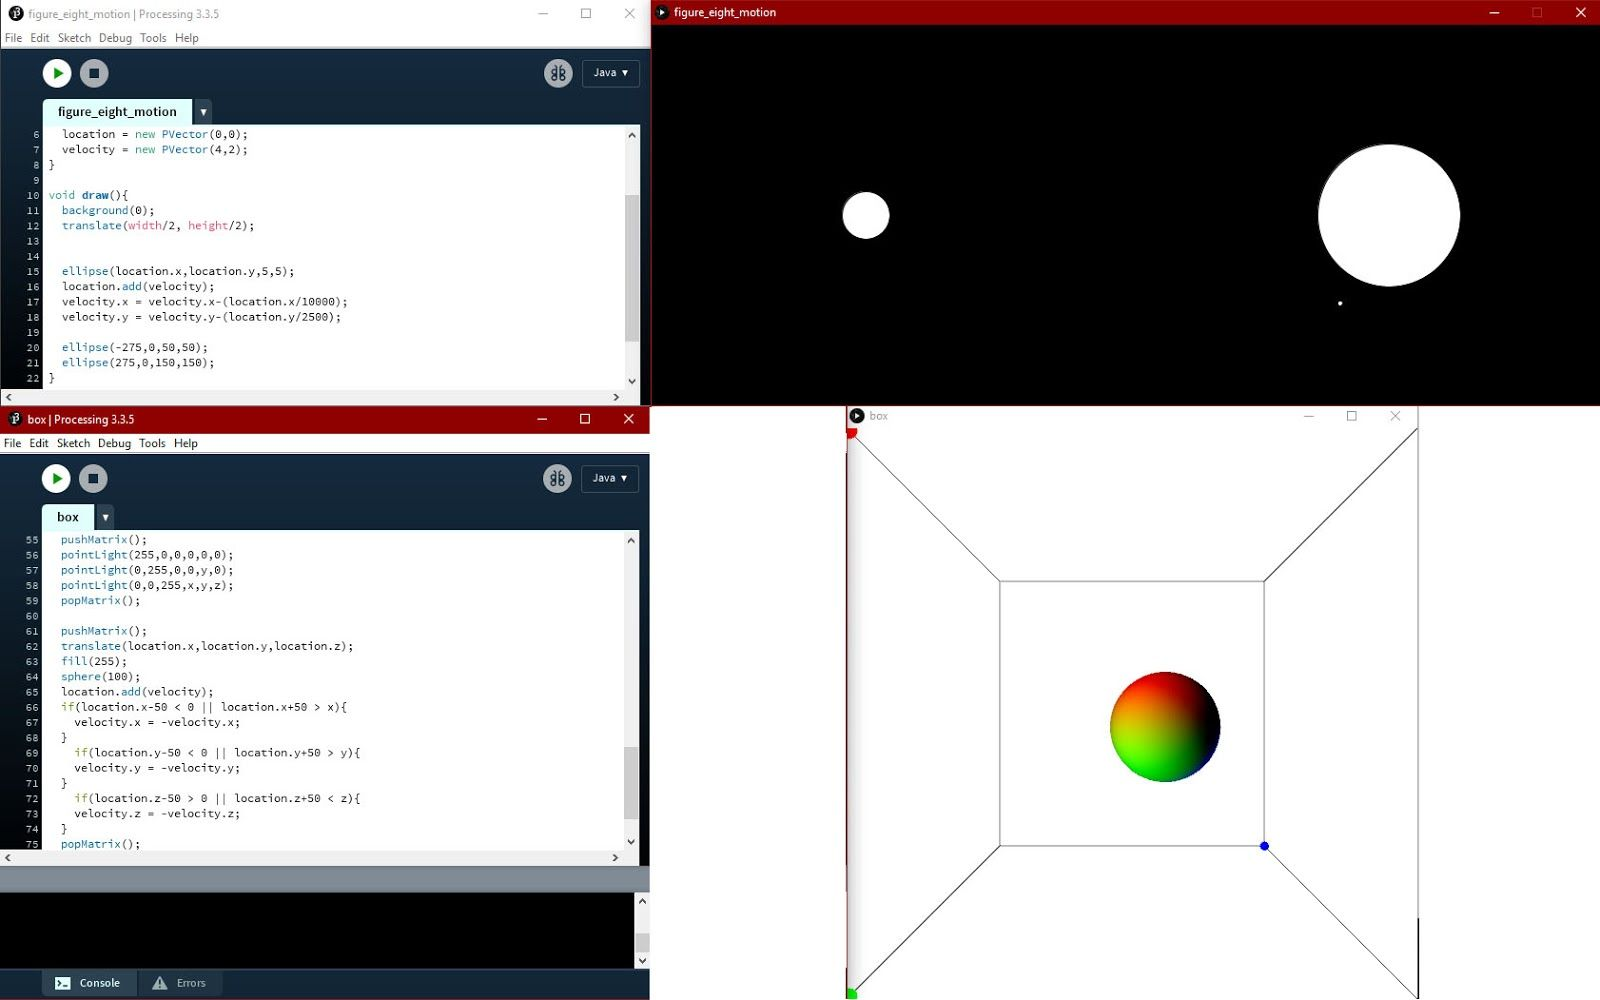
\includegraphics[width=\linewidth]{images/early_proto.jpg}
  \caption{Early prototyping and 3d modelling in Processing}
  \label{fig:early_proto}
\end{figure}

The most recent release of JavaScript at the point of development is JavaScript ES6, based on the ECMA International standard for ECMAScript 6 (ES6). This has enjoyed support across most desktop browsers as of March 2017 \cite{zaytsev_ecmascript_2017}. Two major benefits of using ES6 are the java-like syntax for object instantiation using classes and the availablility of variables with a block scope. Previous versions of JavaScript only used global variables whereas with the inclusion of 'let' in addition to the traditional 'var', the scope of a variable can be limited to a single code block, after which it is discarded. This also helps resolve some issues to do with JavaScript loops requiring arbitrary 'hacks' to avoid problems with enclosure.


\subsubsection{WebGL and three.js}
To provide for a complex graphical output in a web browser it was decided to use the Web Graphics Library (WebGL) capabilities of the HTML canvas element. This would allow the display of either 2-dimensional or 3-dimensional content that uses Open Graphics Library for Embedded Sysems (OpenGL ES) instructions to make the most of any available hardware acceleration through the client's Graphics Processing Unit (GPU).

The syntax for creating graphical primitives (e.g. spheres, cubes) in WebGL is relatively complex for a small return, involving the separate declaration of a number of variables before creating the object itself. It is also quite difficult to optimise for performance with a large number of simple missteps in coding practive that could cause major issues with resultant framerates.

A number of different JavaScript libraries which provide interfaces to simplify the use of WebGL are available. One of the more potent and extensively supported of these is the three.js library \cite{cabello_three.js_????}. It was decided to use three.js to the extent that it provides predifined objects that take constructor arguments to create elements such as spheres, lights and cameras to build a 3-dimensional output in WebGL.

\subsection{Architecture}

The architecture of the delivery platform follows the standard client-server model found in a basic web hosting service. The product was structured to form a one off delivery of all code to the client machine at the time of the initial HyperText Transfer Protocol (HTTP) GET request to the game server. There is no need for extended communication between the client and server beyond this point as there is no need for access to server hosted information. All game logic and data is included in the Javascript source file. In fact any such requirement would introduce needless complexity and performance restrictions. This does make the game simple to 'hack' but, given that there are no negative risks involved in someone accessing the source code, no highscore tables and no multiplayer element, this is of no concern.

JavaScript is typically included as a single file, rather than broken down into individually localised code blocks in separate files. This is to save on request overheads and reduce server load as each HTML page, once parsed, triggers a number of asset requests for any content referred to in the file. Most usually these requests are for one or more CSS files, any embedded images and any embedded scripts. Each individual request has to travel to the server and wait in a queue to be picked up by a worker thread in the server software, thus adding more wait time until the page is ready to be fully rendered on the client. Serving the JavaScript as a single file where possible minimises this delay.

The aim was to include a single file for each of the HTML, CSS and JavaScript items, with allowance made for any libraries and image assets. Bandwidth limitations were determined to be those imposed by 'high speed' internet connections i.e. ADSL2+, 4G or faster. In practice this would mean that transfer speeds would allow for file sizes in the MegaByte range, although all effort would be made to reduce assets sizes where possible by using lossy compression algorithms for the images and minifying any large body of javascript. 'Minifying' is the term given to reducing file sizes by, at the most basic level, removing comments and whitespace characters or going as far as replacing longer, meaningful variable names with short alphanumeric sequences.

The architecture does not quite follow an Model View Controller (MVC) approach but does strive to seperate structure, presentation and logic elements into the HTML, CSS and JavaScript respectively.

\section{Implementation and testing}
\markboth{Implementation and testing}{Implementation and testing}

\subsection{Data types and structures}
The main data types in use in Solar System Explorer are the primitives boolean, number and string and the non-primitive object.

Although these are common to most programming languages, it is worth noting that all numbers in ECMAScript are 64-bit doubles and any floating point values lack the precision of an integer format. This is important to understand as the numbers involved in calculations when it comes to the physics of the solar system can reach beyond the range at which the integer representation is exact. This was notable at times when testing functions in isolation where a trigonometric transformation would return a non-integer result when an integer was expected (e.g. a value of 1.000000000001 as opposed to 1).  Whilst the project requires a good representation of reality it does not require the level of exactitude that an engineering project might so minor deviations were overlooked in this case, but calculations sometimes had to be double checked as what seemed like an inconsequential rounding error was actually  indicative of an error in the order of logic.

One benefit of the use of JavaScript ES6 for a developer with a background in Java programming is the class based instantiation of objects in place of the previously standard prototype model. This allowed for the creation of 5 classes to handle the game logic and allow for the 3D graphical model: Resource, UpgradeEvent, StellarObject, Anchor and Orbit.

The Resource and UpgradeEvent classes create the Objects for the incremental game logic.

A Resource object has properties for the amount of a particular resource that is available at any given time and the rate of change for that resource, along with simple methods for increasing the amount by a value passed as a parameter or increasing the rate of change. There are no negative changes to the values as this is a core feature inherent to incremental game design.

The UpgradeEvents are a set of objects which are continuously checked for pre-requisite conditions which, when met, trigger the visibility of upgrades and store the costs of said upgrades alongside any flavour text that needs to be displayed as and when the event becomes visible.

The Anchor, Orbit and StellarObject classes are used to generate the visual display of the solar system in the 3-dimensional canvas element.

An anchor is a common feature in any system of 3D representation, sometimes referred to as null objects. They are a reference to a point in the 3D space with an x,y and z coordinate and values for rotation about the axes. These are most often used as positional references by which to parent other objects or act as 'control points' in kinematic animation systems.

The Orbit class takes data common to the scientific description of an orbit about a point (e.g. radius, eccentricity, period, etc.), stores those properties in a manner most useful for further calculation and display (e.g. converting input angles given in degrees to radians, automatically calculating the aphelion and perihelion values) and provides an update method which allows for animation of an object around the orbit by incrementing a theta value. This update method includes rotational transformation in 3D space and is discussed in futher detail in the next subsection.

The StellarObject class has properties representing the metadata for any object in space. In the demonstration content at the point of delivery, this was used to generate the Sun and the planets, however it could also be used to provide data for any object in the scene. One iteration used this class to generate moons for the planets. However, given that the relative orbital rotation of the moons was so fast as to make them practically invisible, they were removed for the time being.

In future iterations these 3 classes could be used to generate objects that appear in response to user input (i.e. purchasing upgrades).

JavaScript ES6 is the first release to contain pre-defined collections in the form of maps and sets. These were investigated as potential data structures for the objects instantiated by the above classes, however it was discovered that the performance of these implementations is far slower in current web broswers than using baseline JavaScript when performing lookups \cite{decker_six_2017}. For this reason and the fact that data will not be added by users from outside of the program itself it seemed most sensible to work with simple arrays of objects rather than add the complication of implementing abstract data types. The largest collection of data in the game is the array of upgrade events, but this requires constant interation over the objects to make conditional checks against the pre-requisite event values, so the performance gains from using a data structure with a different method of retrieval would likely be marginal, even if it were faster at finding any single entry (e.g. utilising a hash table).

\subsection{Example method - rotation in 3D space}

\begin{figure}[h!]
  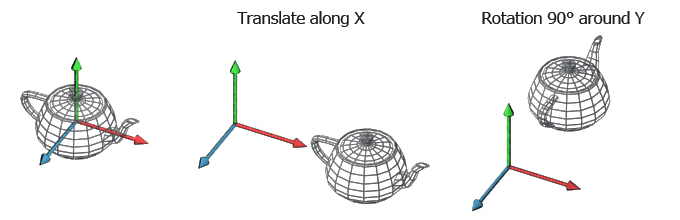
\includegraphics[width=\linewidth]{images/teapot.png}
  \caption{A 'teapot primitive' rotating around the y-axis in 3D space {\cite{_coding_????}}}
  \label{fig:teapot}
\end{figure}

The model used in WebGL for mapping objects in 3-dimensional space is a cartesian coordinate system with an x, y and z value describing any single point. Most data that describes the movement of astronomical bodies is given as a series of angles and distances from a point of rotation as they are usually ellipses or parabola.

To translate from the information given in the physics to that required by the program involves the use of trigonometry. At a basic level, e.g calculating the x and z values for a point on a circle on the x,z plane, this is a relatively simple application of the formulae:

\[x = radius*\sin\theta\]
\[z = radius*\cos\theta\]

In an ellipse centred at its origin the radius is subsituted for the semi-major and semi-minor axis values, in astrophysics terminology these are the equivalent of the aphelion and perihelion, terms which describe the closest and furthest orbital distance from the parent body. (Note that this is only true for orbits where the centre and eccentricity of the ellipse are such that the aphelion and perihelion are perpendicular)

\[x = aphelion*\sin\theta\]
\[z = perihelion*\cos\theta\]

However, most orbits exist at an incline to the ecplitic, a term used for the plane which is coplanar with the orbit of the Earth around the Sun. They are also not all uniformly rotated in relation to the Sun. This necessitates the inclusion of the ability to rotate the orbital ellipse about each of the 3 axes.

\begin{figure}[h!]
  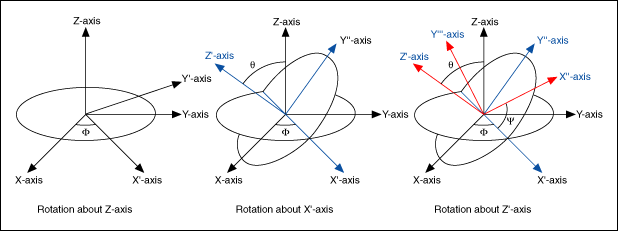
\includegraphics[width=\linewidth]{images/3dcartrot.png}
  \caption{Rotation of an ellipse in 3D space {\cite{_3d_2011}}}
  \label{fig:cartrot}
\end{figure}

Rotation of a point about an axis by a value ($\theta'$) given in radians requires application of the following formulae \cite{acm_siggraph_education_committee_3d_2005}. 

Rotation about the x axis:
\[z' = y*\sin\theta' + z*\cos\theta'\]
\[y' = y*\cos\theta' - z*\sin\theta'\]

Rotation about the y axis:
\[x' = z*\sin\theta' + x*\cos\theta'\]
\[z' = z*\cos\theta' - x*\sin\theta'\]

Rotation about the z axis:
\[y' = x*\sin\theta' + y*\cos\theta'\]
\[x' = x*\cos\theta' - y*\sin\theta'\]

These can be applied consecutively if there is a requirement to rotate about more than one axis.

\bigskip
When coded as a part of the update() method in the Orbit object care had to be taken not to overwrite previous x,y and z values until they were ready for assignment, so some temporary variables with a block scope were included for instantiation within each conditional check for rotation. Simple addition of the coordinates of any parent orbit allowed for rotation of chains of parent and child objects. If no parent was defined or there was no need for the parent to be an Orbit itself, a simple Anchor object could substitute.

\newpage

\begin{lstlisting}[label=Implemented code for rotation in 3D space, caption=Implemented code for rotation in 3D space on an update() call, captionpos=b]
class Orbit {

	[...]
	
	update() {
		// Rotate the value of theta by one measure
		this._theta += this._deltaTheta;
		// calculate the basic x,y,z cartesian coordinates
		// assuming we start by generating on a plane level with the sun->earth axis
		let localX = (Math.sin(this._theta)*this._aphe);
		let localZ = (Math.cos(this._theta)*this._peri);
		let localY = 0;
		// Rotate the coordinates based on the rotation of the orbit around its parent
		if(this._rotX!==0){
			let temp_z = (Math.sin(this._rotX)*localY) + (Math.cos(this._rotX)*localZ);
			let temp_y = (Math.cos(this._rotX)*localY) - (Math.sin(this._rotX)*localZ);
			localZ = temp_z;
			localY = temp_y;
		}
		if(this._rotY!==0){
			let temp_x = (Math.sin(this._rotY)*localZ) + (Math.cos(this._rotY)*localX);
			let temp_z = (Math.cos(this._rotY)*localZ) - (Math.sin(this._rotY)*localX);
			localX = temp_x;
			localZ = temp_z;
		}
		if(this._rotZ!==0){
			let temp_y = (Math.sin(this._rotZ)*localX) + (Math.cos(this._rotZ)*localY);
			let temp_x = (Math.cos(this._rotZ)*localX) - (Math.sin(this._rotZ)*localY);
			localY = temp_y;
			localX = temp_x;
		}
		this._x = localX + this._parent.getX();
		this._z = localZ + this._parent.getZ();
		this._y = localY + this._parent.getY();
	}
}
\end{lstlisting}

\newpage

\subsection{Modelling the planets of the solar system using three.js}
Real data about the solar system and the bodies within were drawn from a number of sources, including directly from NASA factsheets \cite{nasa_planetary_2017}. These were then built into arrays of objects, the properties of which were used to generate scale spherical primitives to represent each of the planets in turn by looping through said array.

\begin{lstlisting}[label=Instances of the StellarObject class, caption=The planets as instances of the StellarObject class, captionpos=b]

// Planets
/*
Params: name, type, diameter(1000s of km to 2sf), orbitalRadiusAu(AU to 1 dp), orbitalRadiusKm (1000s of km), period(relative to 1 earth year), eccentricity, inclination(degrees), axial tilt, axial rotation(relative to 1 earth day)
*/

let sol = new StellarObject("Sol", "Star", 1390, 0, 0, 0, 0, 0, 0, 0);

var planets = [];
let planetMercury = new StellarObject("Mercury", "Terrestrial", 3.0, 0.4, 57900, 0.241, 0.208, 7.00, 0, 59);
planets.push(planetMercury);
let planetVenus = new StellarObject("Venus", "Terrestrial", 7.5, 0.7, 108200, 0.615, 0.007, 3.39, 177, 243);
planets.push(planetVenus);

\end{lstlisting}

This loop uses the three.js library to create primitive spheres with a basic Phong shading model and apply textures from a local image folder.  The textures used for the planets and the Milky Way are taken from NASA and ESO photographic image libraries.


\begin{lstlisting}[label=Loop using three.js objects and methods to create planetary spheres, caption=Loop using three.js objects and methods to create planetary spheres, captionpos=b]

for (let i=0, len=planets.length; i<len; i++) {
	let planetGeometry = new THREE.SphereGeometry((planets[i].getDiameter()/2), 64, 64);
	let planetMap = new THREE.MeshPhongMaterial();
	planetMap.map = THREE.ImageUtils.loadTexture("images/" + planets[i].getName().toLowerCase() + "map.jpg");
	planetMaps.push(planetMap);
	planetModels[i] = new THREE.Mesh(planetGeometry, planetMaps[i]);
	planetModels[i].rotateZ(planets[i].getAxialTilt()*(Math.PI/180));
	scene.add(planetModels[i]);
}

\end{lstlisting}

Similar processes were followed to model the orbits that these planetary spheres were assigned to. The whole 3D interface in the application is a single 3D model, built to scale using these methods, that is simply viewed from different positions by altering the camera's location in the scene.


\subsection{Unit, prototype and integration testing}

There are limited options available when it comes to automated or scripted unit testing for JavaScript. With such a fast moving language, which often uses proprietary frameworks and libraries that virtually constitute domain specific languages (DSLs), it can be difficult for developers of test suites to keep up with the latest trends.
The most tried and tested method appears to be maually unit testing i.e. isolating a block of code, be it a function, method or full script and create another short piece of JavaScript to test for the expected return by outputting this to the console \cite{zaefferer_introduction_2012}.

For segments of the program where the output was not immediately verfiable as correct, e.g. when performing rotational translation as in the previous section, the method of testing was to save the function into a separate .js file, provide sample inputs and check for the correct outputs by sending them to the console in versions of both the Chrome and Firefox browsers on both machines that formed the test bed (One mid-range Core i5 laptop, one high-end Core i7 desktop).

Most of the functionality behind the game logic in this program is simple arithmetic and thus testing was usually not required. Methods that merely incremented a value or performed an addition operation were assumed to be working as expected.

The most challenging parts of the code were those that defined the behavour of on screen elements and that captured user interaction, neither of which can be fully verified using unit testing scripts. Technically mouse clicks can be simulated, but the effort required to do so and adequately measure correct outputs would mean that the main body of the project would become about writing automated tests rather than producing a game. An automated test cannot, for instance, tell you whether a texture has rendered on the surface of a sphere, wrapping in the correct direction or judge the correct opacity of a translucent background.

Most of these elements were tested by building prototypes that modelled the correct behaviour prior to integrating them into the main body of the program. For example in the first 5 weeks of development, the WebGL code for the 3D section of the UI was developed in a separate file structure, away from the game logic.

Integration tests were done using the traditional games development technique of play-throughs as a part of the quality assurance phase \cite{chandler_game_2009}. This is one clear way in which the development lifecycle of a game differs significantly from that of office applications or data-processing applications. At the point of integration specific non-functional behaviours were verified, such as the ability to render the animation at a consistent framerate on a mid-range PC and the legibility of text imposed over the image of a starfield.

\subsection{Acceptance testing}

A body of 13 users volunteered to assist with acceptance testing. Given that the product has no clearly defined audience demographic, these were left to self select into participation by clicking a link that automatically appeared in the user-interface at the end of a play-through.

The users were asked to complete a very short multiple choice questionnaire which related specifically to the aspirational goals of the product. They were subsequently invited to leave free-form comments relating to both the product and to elaborate on their multiple choice answers. This was done via a Google Form which automatically added responses to a speadsheet and generated graphical reports demonstrating the results.

\section{User interface}
\markboth{User interface}{User interface}

Creating the user interface for Solar System Explorer was a 4 stage process. Firstly evaluating the conventions of the genre to ensure that the very first gameplay requirement (GPNFR001) was met, secondly considering general web, graphic design and usabilty conventions and thirdly considering the aesthetic of the inteface given the subject material in question. These findings were then integrated into the final user interface delivered as part of the product.

\subsection{Incremental game conventions}

Multiple games were reviewed from lengthy listings at websites such as Kongregate and Clicker Games, this report will simply summarise a few examples of the findings and how they were used.

\subsubsection{Wireframe layouts}

Most incremental games are designed with a single page layout, a few included pop-up, pop out or tab style menus, but largely the convention of the genre is to encapsulate the entire game in a single screen. With one or two notable exceptions the layout of the user interface is build on a grid system, similar to most print or text-based web design. This is understandable as the platform and the underlying expectations of its rendering capabilities are evolved from the presentation of documents.

This means that most incremental game interfaces can be broken down into a wireframe of their grid and box layout. Following this convention made it possible to create a working product without having to spend an overtly long period trying to position elements on screen and also made it easier to create a responsive layout that changes in line with the viewport window of the web browser software.

\begin{figure}[h!]
  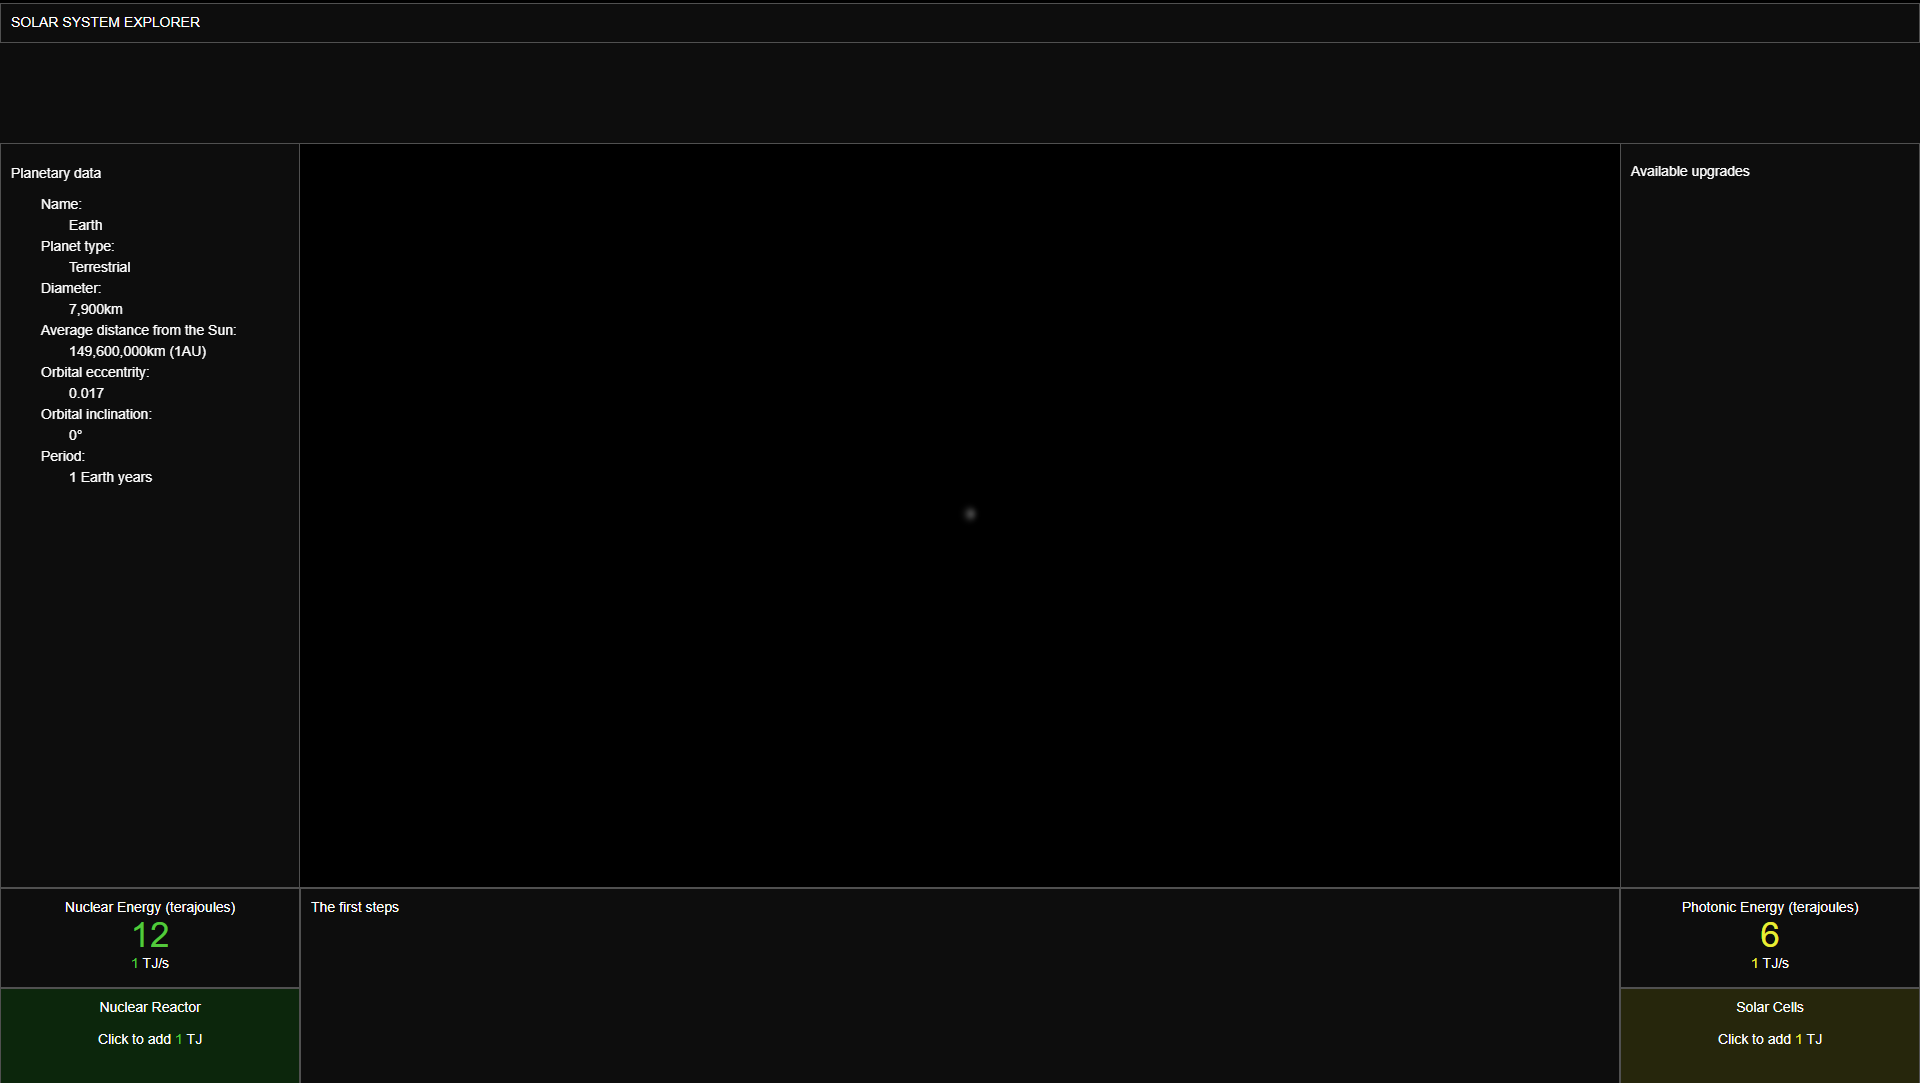
\includegraphics[width=\linewidth]{images/grid_layout.png}
  \caption{An early wireframe grid layout prototype for Solar System Explorer}
  \label{fig:grid_layout}
\end{figure}

\subsubsection{Numeric formatting}

The incrementing numerical values are commonly displayed in a localised format with numeric seperators (commas in the UK).

Numbers are also given as integers, regardless of the actual calculated value, even when representing monetary values.



\subsubsection{Placement of typographic elements}

Text is used to build context and explain the options available for increasing the rate of resource gain. This is represented in one of three ways; delivered as a part of a narrative story in a separately framed on-screen area, as achievements or unlocks in their own free floating puff-boxes or as 'floating text' which appears on screen as an overlay on another graphical element without a bounding box of its own. Floating text also tends to be animated to travel in a pattern and is usually only present on the screen for a brief period.

\subsubsection{Art style}

The two art styles most common in incremental games are cell-shaded cartoon animation style (this includes anime art) and 'pixel art' i.e. deliberately pixelated imagery simulating the low resolution graphics of computing in the 1970s and 80s. Solar System Explorer is definitely an outlier in the decision not to follow this genre convention, but given that a primary requirement is realistic visual representation then to do so would have been counter productive to the goals of the project.

\subsection{General UI conventions}

\subsubsection{Pointer behaviour and signposting interactivity}

It is commonly understood from years of design convention that changing the cursor type of a pointer as it hovers above an element is an indication of interactivity, though this is sometimes misunderstood as affordability \cite{norman_affordance_1999}. However there are arguments that this alone is not enough of an signpost and that ensuring that interactive elements in a user interface also change visually in a 'hover' state is required for clarity. These conventions are in flux as more and more digital interaction is done through touchscreen computing \cite{inostroza_usability_2012}, however in a typical desktop environment they are still a standard.

\subsubsection{Typographic elements}

Typography is an area that has recieved a lot of attention when it comes to display in a web browser, especially given the primary focus on delivering documents. There have been numerous studies and numerous debates amongst publishers, web designers and coders as to what is the most effective way to display text on screen for years.

Some conventions are now well understood. Text should generally appear on screen as having a moderate size and weight, similar to that used in print design, utilise sans-serif typefaces and be displayed at an optimal columnar width for readability \cite{lupton_type_2014}. Solar System Explorer follows these conventions to a reasonable degree, implementing at least the most basic elements. Any short comings are reviewed in the discussion section of this report.

\subsection{Aesthetic}

Albeit that the game interface is a work of design, it still needed to convey a sense of appropriate aesthetic for the theme of space exploration. The field of science fiction is replete with imaginative interpretations of what space ships and space travel look like, from the baroque stylings of H.R. Geiger to the colour coded galaxy of Gene Roddenberry's Star Trek (created under the supervision of art director Matt Jefferies).

None have been so influential as the artwork in Stanley Kubrick's 2001: A Space Odyssey, released in April 1968. Kubrick and art director John Hoesli were said to have been massively inspired by the artwork of  NASA illustrator Harry Lange \cite{sinclair_man_2016} and indeed Lange ended up working on the film project alongside them.

It is from Lange's work, which itself was rooted in providing a sense of realism to a work of fiction, that many conventions of the genre were born. White panels with black heat shielding, exposed sensor and radio arrays, designs that avoided the all too common conventions of 'WWII in space' and so on. In fact, even referring back to Geiger and Jeffries, you can see the lasting impact of Lange's vision in their work. 

\begin{figure}[h!]
  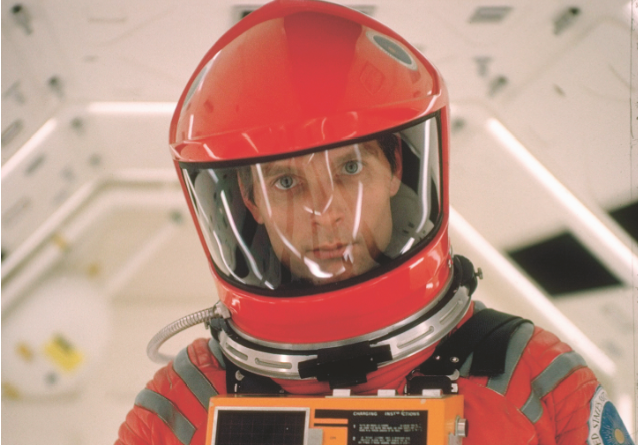
\includegraphics[width=\linewidth]{images/2001_palette.png}
  \caption{The colour palette of 2001: A Space Odyssey {\cite{sinclair_man_2016}}}
  \label{fig:2001_palette}
\end{figure}

Lange's art reflected engineering practice and the similarities between his work and even modern endeavours in space exploration are remarkable. One of the films most lauded for its realism in recent years is 2015's The Martian, which again uses a palette and style that draws on both actual technologies and on Lange's artistic conventions for its speculative imagery. The rotating section of the Hermes spacecraft modelled on the same principles of artificial gravitation as 2001's Space Station 5.

\begin{figure}[h!]
  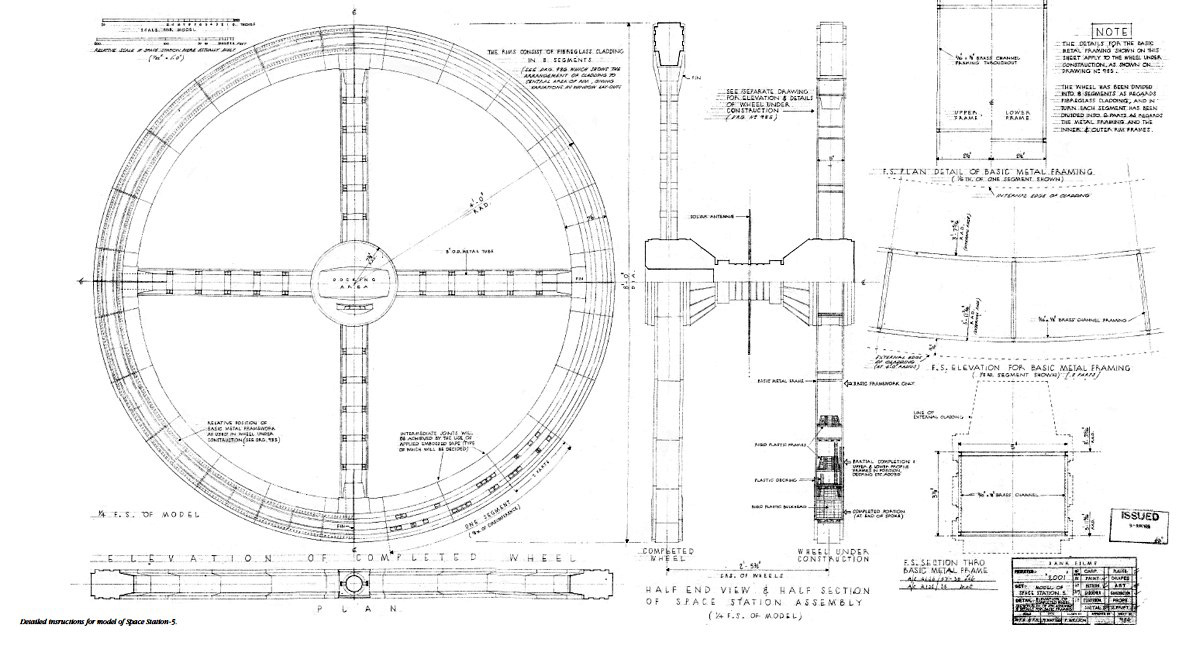
\includegraphics[width=\linewidth]{images/spacestation.jpg}
  \caption{Lange's designs for Space Station 5 from 2001: A Space Odyssey {\cite{sinclair_man_2016}}}
  \label{fig:spacestation}
\end{figure}

To ensure consistency with genre convention Solar System Explorer also borrows from Lange's work in both its pallette and in the graphical flourishes that detail its user interface.

\subsection{Solar System Explorer UI design process}

The design process for Solar System Explorer took a conventional route, moving rapidly from paper prototyping and sketches to developing potential layout wireframes in HTML and CSS, then adding basic functional elements and finally refining the look and feel of the application by adding purely aesthetic elements.

It was decided that the adoption of a widescreen style of presentation for the 3D graphical element would add a slightly cinematic feel to the finished product, therefore interface bars were added at the top and bottom of the screen forcing a widescreen aspect ratio regardless of the size of the browser viewport. These would only become visible after the game's tutorial and, prior to that point, could be used as a blank area onto which instruction or narrative text could be overlaid.

\begin{figure}[h!]
  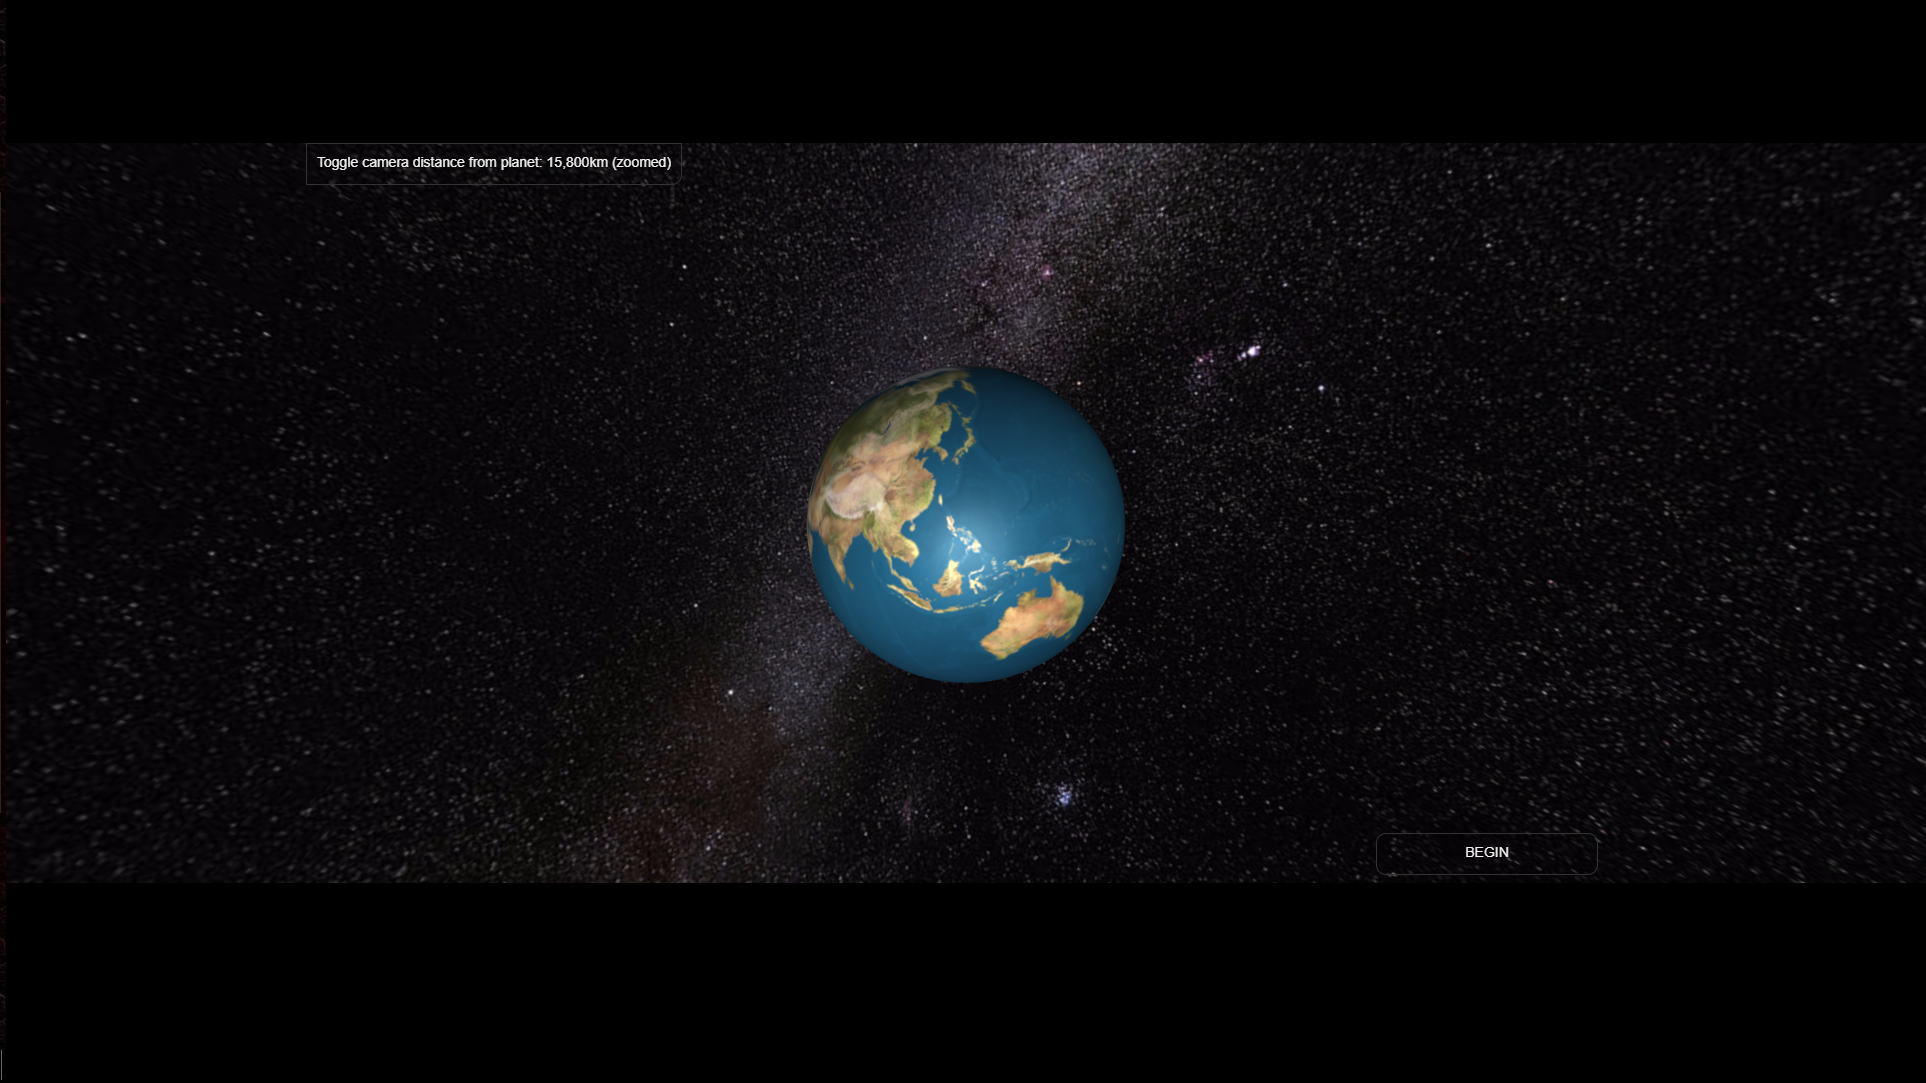
\includegraphics[width=\linewidth]{images/cinematic.png}
  \caption{Cinematic aspect ratio: The opening screen for Solar System Explorer}
  \label{fig:cinematic}
\end{figure}

A common convention of the genre is to place interactive buttons on the far left and right of the screen. Solar System Explorer follows this model, but when showing the 'System View' which shows the position of the planets relative to the sun along with ellipses reprenting their orbits, these side bars retreat off screen.

\begin{figure}[h!]
  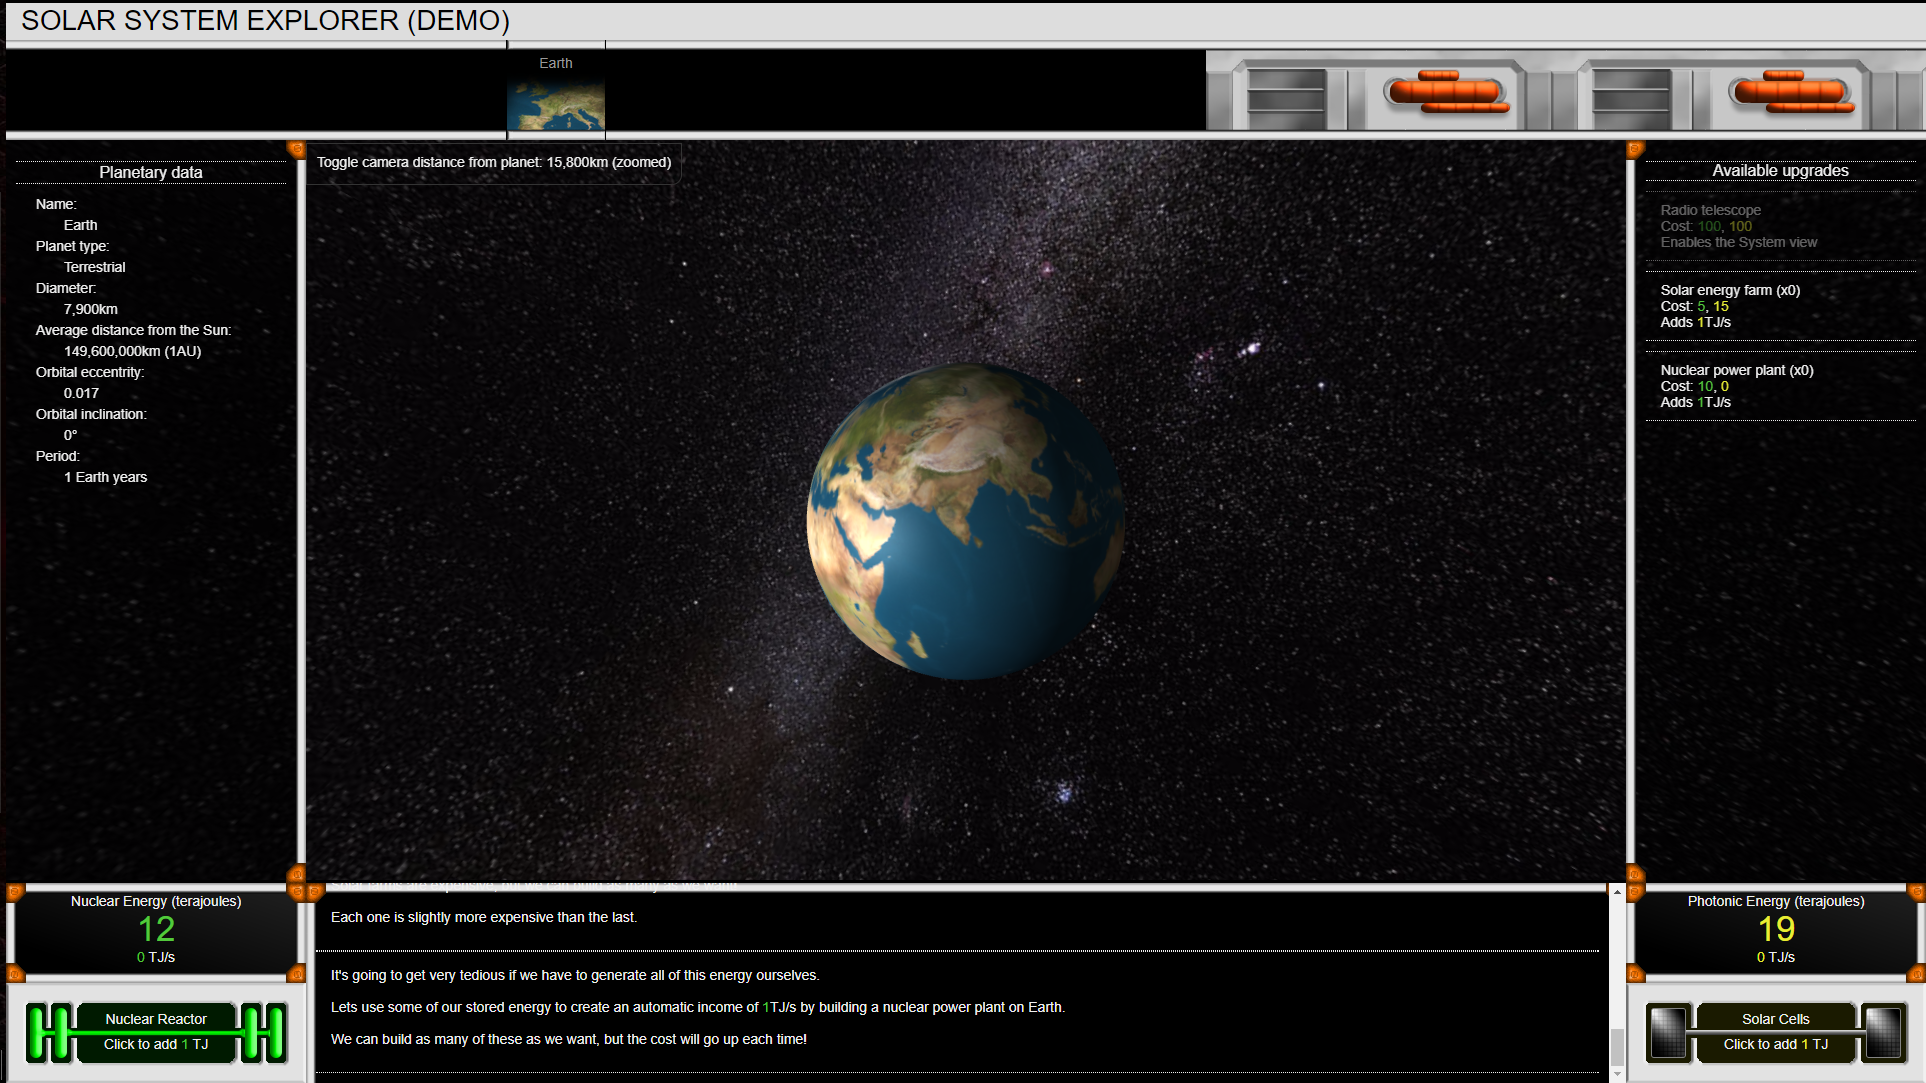
\includegraphics[width=\linewidth]{images/ui_upgrades.png}
  \caption{The planetary UI with available upgrades}
  \label{fig:ui_upgrades}
\end{figure}

All 2D graphical elements were generated in Adobe Photoshop, saved locally and are included in the UI through the use of the CSS:background property.


\section{Project management}
\markboth{Project management}{Project management}

\subsection{Software development lifecycle}
At the very initial stages of the project, when assembling the proposal document, it was noted that game development did not typically follow one of the many formal software development lifecycles (SDLCs) in any strict sense \cite{ramadan_game_2013}. In fact a systematic review published in the Journal of Software Engineering Research and Development found that there was a very poor understanding of the process of game development outside of the 'production phase' (typically referred to as implementation in other SDLCs).

In the case of Solar System Explorer an iterative, incremental approach was taken, with small scale deliverables developed as individual tasks on a day-to-day basis in the style of Agile methodologies.

An overall aspirational goal was set at the initiation of the project as to what the final product may look like and how it may function, with a fallback position if this proved to be too time consuming or complex to produce in the time given. Certain aspects of the product were developed in short bursts, switching between themed streams e.g. Developing a method to dynamically add listeners and event handlers to interface objects for one half day, followed by a further half day creating graphical assets for the user interface.


\subsection{Tools}
A simple set of tasks were stored as a spreadsheet on Google Sheets which allowed for portability and easy annotation. Google Calendar was used to keep track of deadlines, meetings and advisory lectures as well as setting alerts and notifications for said events. Version control for the software itself was implemented using a local git repository which was pushed to the remote repository provided by the school. This was managed through the graphical user interface in the Adobe Dreamweaver integrated development environment (IDE) which was also used as the main editing environment to produce code for the project.

\subsection{Meetings}
Accomodation was made for a weekly meeting with the project supervisor to discuss progress and address any concerns. These would typically last in the region of between 1-2 
hours. These were extremely useful as they allowed for a regular flow of information and provided a motivating factor to achieve a notable level of progress on a weekly basis.

\subsection{Review}
Given that the project resulted in delivery of a product that meets at least the fallback specification then the project management methods would seem to have been generally appropriate in this case. However there was definitely potential for further development of professional practice, for instance there was an over-reliance on documentation through the use of mandated logging which, whilst useful as a summary review of weekly progress, failed to provide a particularly useful tool for the weeks that followed. Completing a simple pro-forma on a daily basis would possibly have resulted in a better measure of progress. Also, a productivity tool that provided better tracking of dates or similar would have been useful in place of the spreadsheet for tracking tasks, be that a free web based application such as Trello or a formal office application like Microsoft Project.

On a project of this size, with only a single developer and a relatively short deadline, it can be quite difficult to appropriately allocate time to administrative and management tasks without either becoming overly bureaucratic and negatively impacting on the production schedule, or ignoring project management tasks to focus solely on implementation. Putting aside a regular slot of 3 hours on a Friday afternoon meant that there was a strict yet simple rule to follow. This also meant that there was a mandatory 'cool down' period at the end of the week in an effort to maintain a standard production schedule, giving time to reflect and step back to gain a broader perspective on the direction of the project.

In the end the production schedule indicated in the project proposal was only loosely followed, but the phases of development roughly approximated the timespans indicated, albeit offset  by a fortnight.


\section{Results and evaluation}
\markboth{Results and evaluation}{Results and evaluation}

Solar System Explorer exists as a software demo, complete as a game framework with some sample content for progress through the game narrative.



The game as it stands mostly fulfils the original general specification. Though it does not meet the aspirational end point of the product, it is far more complete than the state described in the fallback specification. The core mechanics for the incremental game have been realised in full and the 3-dimensional graphical representation of the solar system is complete to a playable degree. Enough game content is present to demonstrate all features of the game mechanics and current features of the user interface.

The numbers increment as expected, upgrade events become visible and trigger properly given the correct prerequisite conditions. Upgrades are purchasable once the resources are available and are listed against specific planets. Purchased upgrades that are one-off events are correctly removed from the interface and those that can be purchased repetitively properly update their costs and display the number of times they have been purchased. The clickable resource boosters work as intended and are modifiable through the purchase of upgrades.

\begin{figure}[h!]
  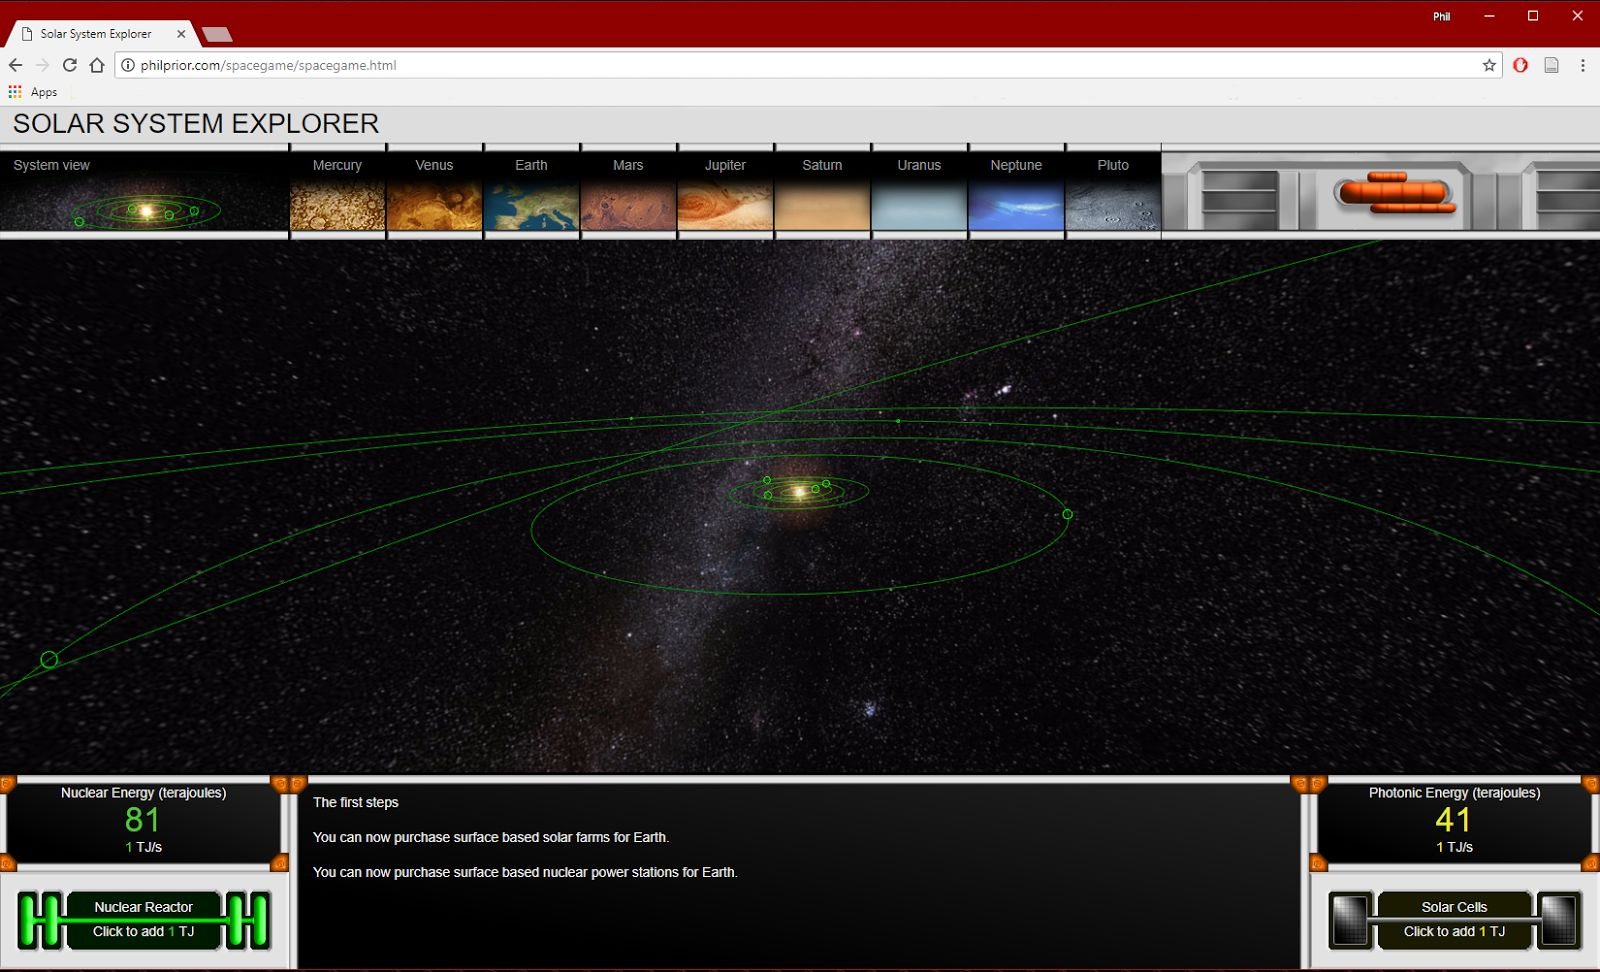
\includegraphics[width=\linewidth]{images/system_view.jpg}
  \caption{System View: Final UI in the Chrome browser}
  \label{fig:system_view}
\end{figure}

The product meets the expected response times specified at the requirements stage, both for initial download and also to user input, once it is running on the client machine.

It is reliable in the sense that at no point does the software appear to critically fail under standard working conditions. After 20+ playthroughs no user has yet reported a crash bug or a technical failure within the game (though one or two  minor issues have been identfied and noted by the developer below).

The product is reasonably robust. If put under stress, e.g. 10+ mouse clicks per second whilst purchasing upgrades, the game can sometimes, but rarely, be forced to report negative values for resources, even though this should be verified in the code at the time of an upgrade purchase. Somehow anindividual event is sometimes 'slipping between' the check for availability and the check for affordability.

The user interface generally behaves in a consistent fashion, though under stress minor misbehaviour can be elicited from the retracting sidebars by rapidly switching back and forth between a planet and the system viewer. This can result in a planet being selected with no sidebars present, though this does not cause any kind of logical failure and a simple repeat click will restore the interface to its normal state.

Of the 13 volunteer users who participated in testing and feedback, all played the demonstration content to completion, 10 of them having played incremental games before. Only 4 reported that they learnt anything new from playing the game, yet one replied in full with "This was a pretty cool way to learn about energy production and space travel. I would have loved to see some links or further facts about space and the planets and the theories around space travel, but I understand this is just a demo. I think it would be a good learning resource for children interested in space. I did enjoy it as an adult." This reflects the lack of narrative content in the demonstration version and the lack of complexity in the scientific information presented.

\begin{figure}[h!]
  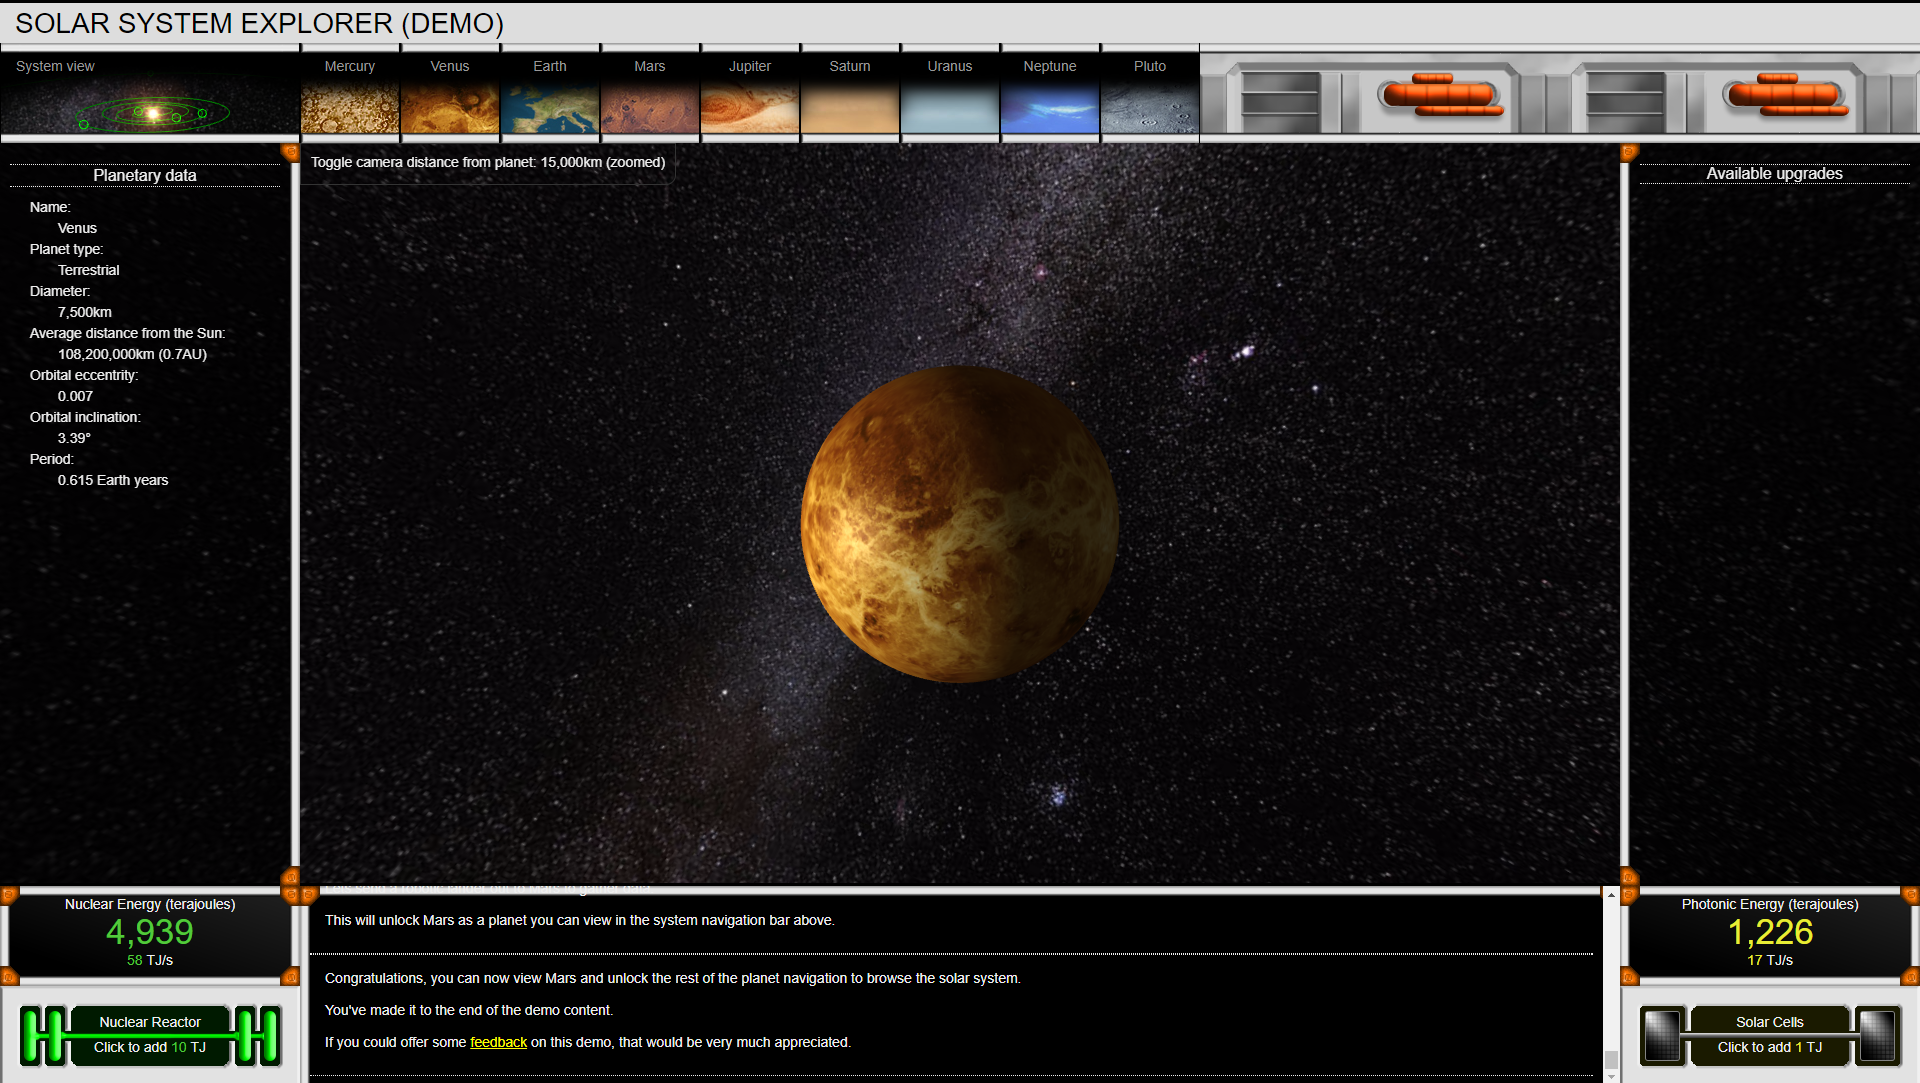
\includegraphics[width=\linewidth]{images/venus.png}
  \caption{Fully unlocked game with a planetary view of Venus}
  \label{fig:venus}
\end{figure}

Offering feedback on the ease of use of the interface, on a 5 tiered ranking of difficulty, 9 of the users ranked the interface at a 1 (the 'easiest' rating) and the rest at a 2. No user found the interface even moderately difficult to use. This is encouraging and suggests that the conventions followed for the interface and any explicit prompts given were adequate to satisfy any non-functional requirements related to learnability. Specific comments were made about the readability of the text area at the base of the interface and about making the availability of new upgrades more obvious by incorporating further visual prompts. Both of these issues are reviewed in the discussion section.

In response to a similarly tiered question ranking the 'realism' of the visualisation (1 representing unrealistic and 5 very realistic) there was a greater spread of results but still with 9 of the 13 choosing to award a rating of 4 or 5. Comments were made about the lack of rings on Saturn and the glossiness of the specular highlights on the gas giants.

Of the 13 respondents the only one to reply negatively when asked if they would be 'interested in playing a full version with more content' did so because "these kind of games [...] eat my life, not because there's anything wrong with it". A testament to the compelling nature of the game genre and also a validation that this implemention was effective enough at employing the psychological 'hooks' and genre conventions in that it reminded the user of 'these kind of games'.

\section{Discussion}
\markboth{Discussion}{Discussion}

One of the test user group stated in their feedback, "More!!! I collected lots of resources I want more! Also a save game feature would be nice, and maybe some online leader boards to add a social or competitive element to the game. Please release the full game!".  This is a good summary introduction to this discussion as it reflects much about the state of the product at this time.

In terms of achievements, Solar System Explorer currently fulfils all mechanical and logical requirements of an incremental game. The programming logic appears to be robust under normal operating conditions, only showing minor bugs when deliberately stressed, none of which cause a catastrophic or critical failure in the running of the program.

The 3-dimensional representation of the solar system is implemented in a fashion that is at least reasonably satisfactory. The orbits demonstrate a good approximation of the actual motion of the planets,  the scales of size and distance are very accurately modelled and the relative rotational speeds are consistent with the actual bodies themselves. The data structures, methods and functions that populate the environment with objects do so capably and deliver performance to a grade expected in this type of application.

The interface is usable, if not refined, and some of the ways in which elements are added and removed using a combination of JavaScript and CSS make the most of the latest developments in those languages. Not to mention features like the dynamic allocation of event listeners to interactive interface elements at the point of becoming available, which keeps the memory footprint of the product lower than it otherwise would be.

This is not to say that the product is without deficiencies. It lacks gameplay content at this point and not enough time was allocated to generating further complexity and depth. In this sense it is hard to justify the suggestion that, in its current state, this game would provide much of an education, save perhaps in those very ignorant of the basic scientific principles and technology. Even then it still falls foul of using shortcuts in the demonstration content to move the experience along quickly, in the reference to 'orbital technologies' for instance.

A save game function as mentioned in the user feedback would have been a great addition and would probably be a key feature in any next iteration.

The costs and prerequisite resource values for the demonstration version are not tuned to provide the most compelling gameplay or give a clear indication of the dilemmas that should be present in choosing to upgrade either one of the resources ahead of the other.

Whilst the data structures used are fast enough and work well for the purposes of this product thus far, the addition of moons and rings, user spawned orbital objects like satellites and a large chain of upgrade events would increase the complexity of the logic and code because of the need to directly address these by their specific positions in their related arrays. With more time it would be preferable to refactor the code to include some form of collection for these objects, be that utilising some features of the inbuilt sets and maps of JavaScript ES6, or proprietary implementations that model similar behaviour.

The user interface could be improved in regards to its readibility, especially the lower section of the UI that incorporates the 'story' element. Perhaps even swapping the position of that information with the less crucial passive data in the left hand retracting sidebar. The animations that fade this information in and out, along with other UI elements could be implemented using a pure JavaScript solution rather than relying so heavily on CSS, however this might mean having to incorporate further premade libraries and frameworks like JQuery. Given enough time the UI should really be subject to a proper usability study.

It was hoped that the 3D visualisation would include text overlays, clickable objects for navigation alongside an animated camera and user feedback in the form of new objects spawned into the environment when upgrades were purchased, however in the window of time for development this proved beyond the capabilities of a developer working with new and unfamiliar languages and libraries. These would definitely be in the plans for a future iteration.

There are other visual refinements that would have been ideal. The Sun's representation as a flare in the system view was implemented in the planetary views in some interstitial stages of development, but this was removed for the final demonstration version as it proved too difficult to reason around a problem where the flare would be rendered in the viewport even when the sun's z coordinate was behind the position of the camera. This led to the odd visual artifact of the Sun appearing to cast both light and shadow on any planets further out from the origin than Jupiter. Adding layered flares that animate as the Sun moved across the viewport to give the impression that the camera is an actual glass lens would have also been a nice effect, but the documentation for the three.js library was not up to date with the current version of the code. It was sadly too time consuming to dig down into the logic of the 44,000 lines of code in the library to figure out how the required callback function would be properly used. With more time shaders could have been added to the Sun and OpenGL post-processing effects like bloom could have given an even more photorealistic feel.

In short, there are many potential future developments for the program. It would have been wonderful to have implemented more of these features and to have a full gameplay experience ready for delivery at project's end. However some of these were defined from the beginning as aspirational goals and should not detract too heavily from the fact that the core aims of the project have been realised in the final product.

\newpage
\section{Conclusion}
\markboth{Conclusion}{Conclusion}

Solar System Explorer is a functionally complete program which simply needs populating with more content to provide a full length game experience and a more in-depth gateway to scientific knowledge and terminology. The interface would definitely benefit from further enhancements yet, taken as a whole, this software is already at the stage where it has the potential to be considered a valid beta release candidate.

It is mechanically complete enough to justify the label 'incremental game' and the core features of the genre have been incorporated into the game's framework. The visual aspect is detailed enough to meet the goals of realism set out in the introduction. It definitely demonstrates a departure from the cartoonish art styles and abstract subject material otherwise common in the field.

Compared against the expectations set out in the introductory sections of this report Solar System Explorer displays a good measure of success as a 'relatively-realistic incremental browser game with an astrophysics theme'.

\section{Sources of submitted code}
\markboth{Sources of submitted code}{Sources of submitted code}
All submitted code with the exception of the three.js library was created by this report's author.

\noindent
Acknowledgement is given to the following for tutorial content, examples and documentation:
\begin{itemize}
\item three.js (threejs.org)
\item Processing (processing.org)
\item w3schools.com
\end{itemize}
Whilst no code was copied verbatim from these sources, each provided a wealth of educational information that assisted with this project.

\addcontentsline{toc}{section}{References}
\printbibliography

\appendix
\appendixpage
\addappheadtotoc

\section{Location and structure of git repository.}

This project's git repository is located at:
\begin{verbatim}
	https://git-teaching.cs.bham.ac.uk/mod-msc-proj-2006/pcp620.git
\end{verbatim}

\noindent
The root directory of the repository contains 4 files and 1 subdirectory that comprise the assets for the application, these being:

\begin{verbatim}
	spacegame.html
	spacegame.css
	spacegamemechanics.js
	three-min.js
	/images (subdirectory)
\end{verbatim}

\noindent
All contents the images directory are required for the application to run as intended.

\bigskip
\noindent
The root directory also contains the subdirectory /report which hosts all of the LaTeX files and image assets used in the creation of this report.


\section{Live inspection location}
For ease of inspection, the product may be viewed on a live web server at:
\begin{verbatim}
	http://philprior.com/spacegame/spacegame.html
\end{verbatim}
Please be sure to use the lastest releases of either the Google Chrome or Mozilla Firefox web browsers to view this application.

\newpage

\section{Image asset licences}

Below are the permissions given for use of the images that form the textures of the planets (NASA) and the wrapping image of the solar system (ESO).

\subsection{NASA Media Usage Guidelines - Still Images and Related Computer Files for Non-Commercial Use}

NASA content - images, audio, video, and computer files used in the rendition of 3-dimensional models, such as texture maps and polygon data in any format - generally are not copyrighted. You may use this material for educational or informational purposes, including photo collections, textbooks, public exhibits, computer graphical simulations and Internet Web pages. This general permission extends to personal Web pages.

News outlets, schools, and text-book authors may use NASA content without needing explicit permission. NASA content used in a factual manner that does not imply endorsement may be used without needing explicit permission. NASA should be acknowledged as the source of the material. NASA occasionally uses copyrighted material by permission on its website. Those images will be marked copyright with the name of the copyright holder. NASA's use does not convey any rights to others to use the same material. Those wishing to use copyrighted material must contact the copyright holder directly.

\subsection{ESO - Usage of images, videos and web texts}

Unless specifically noted, the images and videos distributed from the public ESO web site, along with the texts of press releases, announcements, pictures of the week and captions, are licensed under a Creative Commons Attribution 4.0 International License, and may on a non-exclusive basis be reproduced without fee provided the credit is clear and visible.

\newpage

\section{Framework licence - three.js}

\begin{verbatim}
The MIT License

Copyright © 2010-2017 three.js authors

Permission is hereby granted, free of charge, to any person obtaining a copy
of this software and associated documentation files (the "Software"), to deal
in the Software without restriction, including without limitation the rights
to use, copy, modify, merge, publish, distribute, sublicense, and/or sell
copies of the Software, and to permit persons to whom the Software is
furnished to do so, subject to the following conditions:

The above copyright notice and this permission notice shall be included in
all copies or substantial portions of the Software.

THE SOFTWARE IS PROVIDED "AS IS", WITHOUT WARRANTY OF ANY KIND, EXPRESS OR
IMPLIED, INCLUDING BUT NOT LIMITED TO THE WARRANTIES OF MERCHANTABILITY,
FITNESS FOR A PARTICULAR PURPOSE AND NONINFRINGEMENT. IN NO EVENT SHALL THE
AUTHORS OR COPYRIGHT HOLDERS BE LIABLE FOR ANY CLAIM, DAMAGES OR OTHER
LIABILITY, WHETHER IN AN ACTION OF CONTRACT, TORT OR OTHERWISE, ARISING FROM,
OUT OF OR IN CONNECTION WITH THE SOFTWARE OR THE USE OR OTHER DEALINGS IN
THE SOFTWARE.
\end{verbatim}

\declaration

\end{document}